%
\begin{isabellebody}%
\def\isabellecontext{Examples}%
%
\isadelimtheory
%
\endisadelimtheory
%
\isatagtheory
\isacommand{theory}\isamarkupfalse%
\ Examples\isanewline
\isakeyword{imports}\ Main\isanewline
\isakeyword{begin}%
\endisatagtheory
{\isafoldtheory}%
%
\isadelimtheory
\isanewline
%
\endisadelimtheory
%
\isadeliminvisible
\isanewline
%
\endisadeliminvisible
%
\isataginvisible
\isacommand{pretty{\isaliteral{5F}{\isacharunderscore}}setmargin}\isamarkupfalse%
\ {\isadigit{6}}{\isadigit{5}}%
\endisataginvisible
{\isafoldinvisible}%
%
\isadeliminvisible
%
\endisadeliminvisible
%
\isamarkupsection{Introduction%
}
\isamarkuptrue%
%
\begin{isamarkuptext}%
Locales are based on contexts.  A \emph{context} can be seen as a
  formula schema
\[
  \isa{{\isaliteral{5C3C416E643E}{\isasymAnd}}x\isaliteral{5C3C5E7375623E}{}\isactrlsub {\isadigit{1}}{\isaliteral{5C3C646F74733E}{\isasymdots}}x\isaliteral{5C3C5E7375623E}{}\isactrlsub n{\isaliteral{2E}{\isachardot}}\ {\isaliteral{5C3C6C6272616B6B3E}{\isasymlbrakk}}\ A\isaliteral{5C3C5E7375623E}{}\isactrlsub {\isadigit{1}}{\isaliteral{3B}{\isacharsemicolon}}\ {\isaliteral{5C3C646F74733E}{\isasymdots}}\ {\isaliteral{3B}{\isacharsemicolon}}A\isaliteral{5C3C5E7375623E}{}\isactrlsub m\ {\isaliteral{5C3C726272616B6B3E}{\isasymrbrakk}}\ {\isaliteral{5C3C4C6F6E6772696768746172726F773E}{\isasymLongrightarrow}}\ {\isaliteral{5C3C646F74733E}{\isasymdots}}}
\]
  where the variables~\isa{x\isaliteral{5C3C5E7375623E}{}\isactrlsub {\isadigit{1}}}, \ldots,~\isa{x\isaliteral{5C3C5E7375623E}{}\isactrlsub n} are called
  \emph{parameters} and the premises $\isa{A\isaliteral{5C3C5E7375623E}{}\isactrlsub {\isadigit{1}}}, \ldots,~\isa{A\isaliteral{5C3C5E7375623E}{}\isactrlsub m}$ \emph{assumptions}.  A formula~\isa{C}
  is a \emph{theorem} in the context if it is a conclusion
\[
  \isa{{\isaliteral{5C3C416E643E}{\isasymAnd}}x\isaliteral{5C3C5E7375623E}{}\isactrlsub {\isadigit{1}}{\isaliteral{5C3C646F74733E}{\isasymdots}}x\isaliteral{5C3C5E7375623E}{}\isactrlsub n{\isaliteral{2E}{\isachardot}}\ {\isaliteral{5C3C6C6272616B6B3E}{\isasymlbrakk}}\ A\isaliteral{5C3C5E7375623E}{}\isactrlsub {\isadigit{1}}{\isaliteral{3B}{\isacharsemicolon}}\ {\isaliteral{5C3C646F74733E}{\isasymdots}}\ {\isaliteral{3B}{\isacharsemicolon}}A\isaliteral{5C3C5E7375623E}{}\isactrlsub m\ {\isaliteral{5C3C726272616B6B3E}{\isasymrbrakk}}\ {\isaliteral{5C3C4C6F6E6772696768746172726F773E}{\isasymLongrightarrow}}\ C}.
\]
  Isabelle/Isar's notion of context goes beyond this logical view.
  Its contexts record, in a consecutive order, proved
  conclusions along with \emph{attributes}, which can provide context
  specific configuration information for proof procedures and concrete
  syntax.  From a logical perspective, locales are just contexts that
  have been made persistent.  To the user, though, they provide
  powerful means for declaring and combining contexts, and for the
  reuse of theorems proved in these contexts.%
\end{isamarkuptext}%
\isamarkuptrue%
%
\isamarkupsection{Simple Locales%
}
\isamarkuptrue%
%
\begin{isamarkuptext}%
In its simplest form, a
  \emph{locale declaration} consists of a sequence of context elements
  declaring parameters (keyword \isakeyword{fixes}) and assumptions
  (keyword \isakeyword{assumes}).  The following is the specification of
  partial orders, as locale \isa{partial{\isaliteral{5F}{\isacharunderscore}}order}.%
\end{isamarkuptext}%
\isamarkuptrue%
\ \ \isacommand{locale}\isamarkupfalse%
\ partial{\isaliteral{5F}{\isacharunderscore}}order\ {\isaliteral{3D}{\isacharequal}}\isanewline
\ \ \ \ \isakeyword{fixes}\ le\ {\isaliteral{3A}{\isacharcolon}}{\isaliteral{3A}{\isacharcolon}}\ {\isaliteral{22}{\isachardoublequoteopen}}{\isaliteral{27}{\isacharprime}}a\ {\isaliteral{5C3C52696768746172726F773E}{\isasymRightarrow}}\ {\isaliteral{27}{\isacharprime}}a\ {\isaliteral{5C3C52696768746172726F773E}{\isasymRightarrow}}\ bool{\isaliteral{22}{\isachardoublequoteclose}}\ {\isaliteral{28}{\isacharparenleft}}\isakeyword{infixl}\ {\isaliteral{22}{\isachardoublequoteopen}}{\isaliteral{5C3C737173756273657465713E}{\isasymsqsubseteq}}{\isaliteral{22}{\isachardoublequoteclose}}\ {\isadigit{5}}{\isadigit{0}}{\isaliteral{29}{\isacharparenright}}\isanewline
\ \ \ \ \isakeyword{assumes}\ refl\ {\isaliteral{5B}{\isacharbrackleft}}intro{\isaliteral{2C}{\isacharcomma}}\ simp{\isaliteral{5D}{\isacharbrackright}}{\isaliteral{3A}{\isacharcolon}}\ {\isaliteral{22}{\isachardoublequoteopen}}x\ {\isaliteral{5C3C737173756273657465713E}{\isasymsqsubseteq}}\ x{\isaliteral{22}{\isachardoublequoteclose}}\isanewline
\ \ \ \ \ \ \isakeyword{and}\ anti{\isaliteral{5F}{\isacharunderscore}}sym\ {\isaliteral{5B}{\isacharbrackleft}}intro{\isaliteral{5D}{\isacharbrackright}}{\isaliteral{3A}{\isacharcolon}}\ {\isaliteral{22}{\isachardoublequoteopen}}{\isaliteral{5C3C6C6272616B6B3E}{\isasymlbrakk}}\ x\ {\isaliteral{5C3C737173756273657465713E}{\isasymsqsubseteq}}\ y{\isaliteral{3B}{\isacharsemicolon}}\ y\ {\isaliteral{5C3C737173756273657465713E}{\isasymsqsubseteq}}\ x\ {\isaliteral{5C3C726272616B6B3E}{\isasymrbrakk}}\ {\isaliteral{5C3C4C6F6E6772696768746172726F773E}{\isasymLongrightarrow}}\ x\ {\isaliteral{3D}{\isacharequal}}\ y{\isaliteral{22}{\isachardoublequoteclose}}\isanewline
\ \ \ \ \ \ \isakeyword{and}\ trans\ {\isaliteral{5B}{\isacharbrackleft}}trans{\isaliteral{5D}{\isacharbrackright}}{\isaliteral{3A}{\isacharcolon}}\ {\isaliteral{22}{\isachardoublequoteopen}}{\isaliteral{5C3C6C6272616B6B3E}{\isasymlbrakk}}\ x\ {\isaliteral{5C3C737173756273657465713E}{\isasymsqsubseteq}}\ y{\isaliteral{3B}{\isacharsemicolon}}\ y\ {\isaliteral{5C3C737173756273657465713E}{\isasymsqsubseteq}}\ z\ {\isaliteral{5C3C726272616B6B3E}{\isasymrbrakk}}\ {\isaliteral{5C3C4C6F6E6772696768746172726F773E}{\isasymLongrightarrow}}\ x\ {\isaliteral{5C3C737173756273657465713E}{\isasymsqsubseteq}}\ z{\isaliteral{22}{\isachardoublequoteclose}}%
\begin{isamarkuptext}%
The parameter of this locale is~\isa{le},
  which is a binary predicate with infix syntax~\isa{{\isaliteral{5C3C737173756273657465713E}{\isasymsqsubseteq}}}.  The
  parameter syntax is available in the subsequent
  assumptions, which are the familiar partial order axioms.

  Isabelle recognises unbound names as free variables.  In locale
  assumptions, these are implicitly universally quantified.  That is,
  \isa{{\isaliteral{5C3C6C6272616B6B3E}{\isasymlbrakk}}x\ {\isaliteral{5C3C737173756273657465713E}{\isasymsqsubseteq}}\ y{\isaliteral{3B}{\isacharsemicolon}}\ y\ {\isaliteral{5C3C737173756273657465713E}{\isasymsqsubseteq}}\ z{\isaliteral{5C3C726272616B6B3E}{\isasymrbrakk}}\ {\isaliteral{5C3C4C6F6E6772696768746172726F773E}{\isasymLongrightarrow}}\ x\ {\isaliteral{5C3C737173756273657465713E}{\isasymsqsubseteq}}\ z} in fact means
  \isa{{\isaliteral{5C3C416E643E}{\isasymAnd}}x\ y\ z{\isaliteral{2E}{\isachardot}}\ {\isaliteral{5C3C6C6272616B6B3E}{\isasymlbrakk}}x\ {\isaliteral{5C3C737173756273657465713E}{\isasymsqsubseteq}}\ y{\isaliteral{3B}{\isacharsemicolon}}\ y\ {\isaliteral{5C3C737173756273657465713E}{\isasymsqsubseteq}}\ z{\isaliteral{5C3C726272616B6B3E}{\isasymrbrakk}}\ {\isaliteral{5C3C4C6F6E6772696768746172726F773E}{\isasymLongrightarrow}}\ x\ {\isaliteral{5C3C737173756273657465713E}{\isasymsqsubseteq}}\ z}.

  Two commands are provided to inspect locales:
  \isakeyword{print\_locales} lists the names of all locales of the
  current theory; \isakeyword{print\_locale}~$n$ prints the parameters
  and assumptions of locale $n$; the variation \isakeyword{print\_locale!}~$n$
  additionally outputs the conclusions that are stored in the locale.
  We may inspect the new locale
  by issuing \isakeyword{print\_locale!} \isa{partial{\isaliteral{5F}{\isacharunderscore}}order}.  The output
  is the following list of context elements.
\begin{small}
\begin{alltt}
  \isakeyword{fixes} le :: "'a \(\Rightarrow\) 'a \(\Rightarrow\)  bool" (\isakeyword{infixl} "\(\sqsubseteq\)" 50)
  \isakeyword{assumes} "partial_order op \(\sqsubseteq\)"
  \isakeyword{notes} assumption
    refl [intro, simp] = `?x \(\sqsubseteq\) ?x`
    \isakeyword{and}
    anti_sym [intro] = `\(\isasymlbrakk\)?x \(\sqsubseteq\) ?y; ?y \(\sqsubseteq\) ?x\(\isasymrbrakk\) \(\Longrightarrow\) ?x = ?y`
    \isakeyword{and}
    trans [trans] = `\(\isasymlbrakk\)?x \(\sqsubseteq\) ?y; ?y \(\sqsubseteq\) ?z\(\isasymrbrakk\) \(\Longrightarrow\) ?x \(\sqsubseteq\) ?z`
\end{alltt}
\end{small}
  The keyword \isakeyword{notes} denotes a conclusion element.  There
  is one conclusion, which was added automatically.  Instead, there is
  only one assumption, namely \isa{partial{\isaliteral{5F}{\isacharunderscore}}order\ op\ {\isaliteral{5C3C737173756273657465713E}{\isasymsqsubseteq}}}.  The locale
  declaration has introduced the predicate \isa{partial{\isaliteral{5F}{\isacharunderscore}}order} to the theory.  This predicate is the
  \emph{locale predicate}.  Its definition may be inspected by
  issuing \isakeyword{thm} \isa{partial{\isaliteral{5F}{\isacharunderscore}}order{\isaliteral{5F}{\isacharunderscore}}def}.
  \begin{isabelle}%
\ \ partial{\isaliteral{5F}{\isacharunderscore}}order\ {\isaliteral{3F}{\isacharquery}}le\ {\isaliteral{5C3C65717569763E}{\isasymequiv}}\isanewline
\isaindent{\ \ }{\isaliteral{28}{\isacharparenleft}}{\isaliteral{5C3C666F72616C6C3E}{\isasymforall}}x{\isaliteral{2E}{\isachardot}}\ {\isaliteral{3F}{\isacharquery}}le\ x\ x{\isaliteral{29}{\isacharparenright}}\ {\isaliteral{5C3C616E643E}{\isasymand}}\isanewline
\isaindent{\ \ }{\isaliteral{28}{\isacharparenleft}}{\isaliteral{5C3C666F72616C6C3E}{\isasymforall}}x\ y{\isaliteral{2E}{\isachardot}}\ {\isaliteral{3F}{\isacharquery}}le\ x\ y\ {\isaliteral{5C3C6C6F6E6772696768746172726F773E}{\isasymlongrightarrow}}\ {\isaliteral{3F}{\isacharquery}}le\ y\ x\ {\isaliteral{5C3C6C6F6E6772696768746172726F773E}{\isasymlongrightarrow}}\ x\ {\isaliteral{3D}{\isacharequal}}\ y{\isaliteral{29}{\isacharparenright}}\ {\isaliteral{5C3C616E643E}{\isasymand}}\isanewline
\isaindent{\ \ }{\isaliteral{28}{\isacharparenleft}}{\isaliteral{5C3C666F72616C6C3E}{\isasymforall}}x\ y\ z{\isaliteral{2E}{\isachardot}}\ {\isaliteral{3F}{\isacharquery}}le\ x\ y\ {\isaliteral{5C3C6C6F6E6772696768746172726F773E}{\isasymlongrightarrow}}\ {\isaliteral{3F}{\isacharquery}}le\ y\ z\ {\isaliteral{5C3C6C6F6E6772696768746172726F773E}{\isasymlongrightarrow}}\ {\isaliteral{3F}{\isacharquery}}le\ x\ z{\isaliteral{29}{\isacharparenright}}%
\end{isabelle}
  In our example, this is a unary predicate over the parameter of the
  locale.  It is equivalent to the original assumptions, which have
  been turned into conclusions and are
  available as theorems in the context of the locale.  The names and
  attributes from the locale declaration are associated to these
  theorems and are effective in the context of the locale.

  Each conclusion has a \emph{foundational theorem} as counterpart
  in the theory.  Technically, this is simply the theorem composed
  of context and conclusion.  For the transitivity theorem, this is
  \isa{partial{\isaliteral{5F}{\isacharunderscore}}order{\isaliteral{2E}{\isachardot}}trans}:
  \begin{isabelle}%
\ \ {\isaliteral{5C3C6C6272616B6B3E}{\isasymlbrakk}}partial{\isaliteral{5F}{\isacharunderscore}}order\ {\isaliteral{3F}{\isacharquery}}le{\isaliteral{3B}{\isacharsemicolon}}\ {\isaliteral{3F}{\isacharquery}}le\ {\isaliteral{3F}{\isacharquery}}x\ {\isaliteral{3F}{\isacharquery}}y{\isaliteral{3B}{\isacharsemicolon}}\ {\isaliteral{3F}{\isacharquery}}le\ {\isaliteral{3F}{\isacharquery}}y\ {\isaliteral{3F}{\isacharquery}}z{\isaliteral{5C3C726272616B6B3E}{\isasymrbrakk}}\ {\isaliteral{5C3C4C6F6E6772696768746172726F773E}{\isasymLongrightarrow}}\ {\isaliteral{3F}{\isacharquery}}le\ {\isaliteral{3F}{\isacharquery}}x\ {\isaliteral{3F}{\isacharquery}}z%
\end{isabelle}%
\end{isamarkuptext}%
\isamarkuptrue%
%
\isamarkupsubsection{Targets: Extending Locales%
}
\isamarkuptrue%
%
\begin{isamarkuptext}%
The specification of a locale is fixed, but its list of conclusions
  may be extended through Isar commands that take a \emph{target} argument.
  In the following, \isakeyword{definition} and 
  \isakeyword{theorem} are illustrated.
  Table~\ref{tab:commands-with-target} lists Isar commands that accept
  a target.  Isar provides various ways of specifying the target.  A
  target for a single command may be indicated with keyword
  \isakeyword{in} in the following way:

\begin{table}
\hrule
\vspace{2ex}
\begin{center}
\begin{tabular}{ll}
  \isakeyword{definition} & definition through an equation \\
  \isakeyword{inductive} & inductive definition \\
  \isakeyword{primrec} & primitive recursion \\
  \isakeyword{fun}, \isakeyword{function} & general recursion \\
  \isakeyword{abbreviation} & syntactic abbreviation \\
  \isakeyword{theorem}, etc.\ & theorem statement with proof \\
  \isakeyword{theorems}, etc.\ & redeclaration of theorems \\
  \isakeyword{text}, etc.\ & document markup
\end{tabular}
\end{center}
\hrule
\caption{Isar commands that accept a target.}
\label{tab:commands-with-target}
\end{table}%
\end{isamarkuptext}%
\isamarkuptrue%
\ \ \isacommand{definition}\isamarkupfalse%
\ {\isaliteral{28}{\isacharparenleft}}\isakeyword{in}\ partial{\isaliteral{5F}{\isacharunderscore}}order{\isaliteral{29}{\isacharparenright}}\isanewline
\ \ \ \ less\ {\isaliteral{3A}{\isacharcolon}}{\isaliteral{3A}{\isacharcolon}}\ {\isaliteral{22}{\isachardoublequoteopen}}{\isaliteral{27}{\isacharprime}}a\ {\isaliteral{5C3C52696768746172726F773E}{\isasymRightarrow}}\ {\isaliteral{27}{\isacharprime}}a\ {\isaliteral{5C3C52696768746172726F773E}{\isasymRightarrow}}\ bool{\isaliteral{22}{\isachardoublequoteclose}}\ {\isaliteral{28}{\isacharparenleft}}\isakeyword{infixl}\ {\isaliteral{22}{\isachardoublequoteopen}}{\isaliteral{5C3C73717375627365743E}{\isasymsqsubset}}{\isaliteral{22}{\isachardoublequoteclose}}\ {\isadigit{5}}{\isadigit{0}}{\isaliteral{29}{\isacharparenright}}\isanewline
\ \ \ \ \isakeyword{where}\ {\isaliteral{22}{\isachardoublequoteopen}}{\isaliteral{28}{\isacharparenleft}}x\ {\isaliteral{5C3C73717375627365743E}{\isasymsqsubset}}\ y{\isaliteral{29}{\isacharparenright}}\ {\isaliteral{3D}{\isacharequal}}\ {\isaliteral{28}{\isacharparenleft}}x\ {\isaliteral{5C3C737173756273657465713E}{\isasymsqsubseteq}}\ y\ {\isaliteral{5C3C616E643E}{\isasymand}}\ x\ {\isaliteral{5C3C6E6F7465713E}{\isasymnoteq}}\ y{\isaliteral{29}{\isacharparenright}}{\isaliteral{22}{\isachardoublequoteclose}}%
\begin{isamarkuptext}%
The strict order \isa{less} with infix
  syntax~\isa{{\isaliteral{5C3C73717375627365743E}{\isasymsqsubset}}} is
  defined in terms of the locale parameter~\isa{le} and the general
  equality of the object logic we work in.  The definition generates a
  \emph{foundational constant}
  \isa{partial{\isaliteral{5F}{\isacharunderscore}}order{\isaliteral{2E}{\isachardot}}less} with definition \isa{partial{\isaliteral{5F}{\isacharunderscore}}order{\isaliteral{2E}{\isachardot}}less{\isaliteral{5F}{\isacharunderscore}}def}:
  \begin{isabelle}%
\ \ partial{\isaliteral{5F}{\isacharunderscore}}order\ {\isaliteral{3F}{\isacharquery}}le\ {\isaliteral{5C3C4C6F6E6772696768746172726F773E}{\isasymLongrightarrow}}\isanewline
\isaindent{\ \ }partial{\isaliteral{5F}{\isacharunderscore}}order{\isaliteral{2E}{\isachardot}}less\ {\isaliteral{3F}{\isacharquery}}le\ {\isaliteral{3F}{\isacharquery}}x\ {\isaliteral{3F}{\isacharquery}}y\ {\isaliteral{3D}{\isacharequal}}\ {\isaliteral{28}{\isacharparenleft}}{\isaliteral{3F}{\isacharquery}}le\ {\isaliteral{3F}{\isacharquery}}x\ {\isaliteral{3F}{\isacharquery}}y\ {\isaliteral{5C3C616E643E}{\isasymand}}\ {\isaliteral{3F}{\isacharquery}}x\ {\isaliteral{5C3C6E6F7465713E}{\isasymnoteq}}\ {\isaliteral{3F}{\isacharquery}}y{\isaliteral{29}{\isacharparenright}}%
\end{isabelle}
  At the same time, the locale is extended by syntax transformations
  hiding this construction in the context of the locale.  Here, the
  abbreviation \isa{less} is available for
  \isa{partial{\isaliteral{5F}{\isacharunderscore}}order{\isaliteral{2E}{\isachardot}}less\ le}, and it is printed
  and parsed as infix~\isa{{\isaliteral{5C3C73717375627365743E}{\isasymsqsubset}}}.  Finally, the conclusion \isa{less{\isaliteral{5F}{\isacharunderscore}}def} is added to the locale:
  \begin{isabelle}%
\ \ {\isaliteral{28}{\isacharparenleft}}{\isaliteral{3F}{\isacharquery}}x\ {\isaliteral{5C3C73717375627365743E}{\isasymsqsubset}}\ {\isaliteral{3F}{\isacharquery}}y{\isaliteral{29}{\isacharparenright}}\ {\isaliteral{3D}{\isacharequal}}\ {\isaliteral{28}{\isacharparenleft}}{\isaliteral{3F}{\isacharquery}}x\ {\isaliteral{5C3C737173756273657465713E}{\isasymsqsubseteq}}\ {\isaliteral{3F}{\isacharquery}}y\ {\isaliteral{5C3C616E643E}{\isasymand}}\ {\isaliteral{3F}{\isacharquery}}x\ {\isaliteral{5C3C6E6F7465713E}{\isasymnoteq}}\ {\isaliteral{3F}{\isacharquery}}y{\isaliteral{29}{\isacharparenright}}%
\end{isabelle}%
\end{isamarkuptext}%
\isamarkuptrue%
%
\begin{isamarkuptext}%
The treatment of theorem statements is more straightforward.
  As an example, here is the derivation of a transitivity law for the
  strict order relation.%
\end{isamarkuptext}%
\isamarkuptrue%
\ \ \isacommand{lemma}\isamarkupfalse%
\ {\isaliteral{28}{\isacharparenleft}}\isakeyword{in}\ partial{\isaliteral{5F}{\isacharunderscore}}order{\isaliteral{29}{\isacharparenright}}\ less{\isaliteral{5F}{\isacharunderscore}}le{\isaliteral{5F}{\isacharunderscore}}trans\ {\isaliteral{5B}{\isacharbrackleft}}trans{\isaliteral{5D}{\isacharbrackright}}{\isaliteral{3A}{\isacharcolon}}\isanewline
\ \ \ \ {\isaliteral{22}{\isachardoublequoteopen}}{\isaliteral{5C3C6C6272616B6B3E}{\isasymlbrakk}}\ x\ {\isaliteral{5C3C73717375627365743E}{\isasymsqsubset}}\ y{\isaliteral{3B}{\isacharsemicolon}}\ y\ {\isaliteral{5C3C737173756273657465713E}{\isasymsqsubseteq}}\ z\ {\isaliteral{5C3C726272616B6B3E}{\isasymrbrakk}}\ {\isaliteral{5C3C4C6F6E6772696768746172726F773E}{\isasymLongrightarrow}}\ x\ {\isaliteral{5C3C73717375627365743E}{\isasymsqsubset}}\ z{\isaliteral{22}{\isachardoublequoteclose}}\isanewline
%
\isadelimvisible
\ \ \ \ %
\endisadelimvisible
%
\isatagvisible
\isacommand{unfolding}\isamarkupfalse%
\ less{\isaliteral{5F}{\isacharunderscore}}def\ \isacommand{by}\isamarkupfalse%
\ {\isaliteral{28}{\isacharparenleft}}blast\ intro{\isaliteral{3A}{\isacharcolon}}\ trans{\isaliteral{29}{\isacharparenright}}%
\endisatagvisible
{\isafoldvisible}%
%
\isadelimvisible
%
\endisadelimvisible
%
\begin{isamarkuptext}%
In the context of the proof, conclusions of the
  locale may be used like theorems.  Attributes are effective: \isa{anti{\isaliteral{5F}{\isacharunderscore}}sym} was
  declared as introduction rule, hence it is in the context's set of
  rules used by the classical reasoner by default.%
\end{isamarkuptext}%
\isamarkuptrue%
%
\isamarkupsubsection{Context Blocks%
}
\isamarkuptrue%
%
\begin{isamarkuptext}%
When working with locales, sequences of commands with the same
  target are frequent.  A block of commands, delimited by
  \isakeyword{begin} and \isakeyword{end}, makes a theory-like style
  of working possible.  All commands inside the block refer to the
  same target.  A block may immediately follow a locale
  declaration, which makes that locale the target.  Alternatively the
  target for a block may be given with the \isakeyword{context}
  command.

  This style of working is illustrated in the block below, where
  notions of infimum and supremum for partial orders are introduced,
  together with theorems about their uniqueness.%
\end{isamarkuptext}%
\isamarkuptrue%
\ \ \isacommand{context}\isamarkupfalse%
\ partial{\isaliteral{5F}{\isacharunderscore}}order\ \isakeyword{begin}\isanewline
\isanewline
\ \ \isacommand{definition}\isamarkupfalse%
\isanewline
\ \ \ \ is{\isaliteral{5F}{\isacharunderscore}}inf\ \isakeyword{where}\ {\isaliteral{22}{\isachardoublequoteopen}}is{\isaliteral{5F}{\isacharunderscore}}inf\ x\ y\ i\ {\isaliteral{3D}{\isacharequal}}\isanewline
\ \ \ \ \ \ {\isaliteral{28}{\isacharparenleft}}i\ {\isaliteral{5C3C737173756273657465713E}{\isasymsqsubseteq}}\ x\ {\isaliteral{5C3C616E643E}{\isasymand}}\ i\ {\isaliteral{5C3C737173756273657465713E}{\isasymsqsubseteq}}\ y\ {\isaliteral{5C3C616E643E}{\isasymand}}\ {\isaliteral{28}{\isacharparenleft}}{\isaliteral{5C3C666F72616C6C3E}{\isasymforall}}z{\isaliteral{2E}{\isachardot}}\ z\ {\isaliteral{5C3C737173756273657465713E}{\isasymsqsubseteq}}\ x\ {\isaliteral{5C3C616E643E}{\isasymand}}\ z\ {\isaliteral{5C3C737173756273657465713E}{\isasymsqsubseteq}}\ y\ {\isaliteral{5C3C6C6F6E6772696768746172726F773E}{\isasymlongrightarrow}}\ z\ {\isaliteral{5C3C737173756273657465713E}{\isasymsqsubseteq}}\ i{\isaliteral{29}{\isacharparenright}}{\isaliteral{29}{\isacharparenright}}{\isaliteral{22}{\isachardoublequoteclose}}\isanewline
\isanewline
\ \ \isacommand{definition}\isamarkupfalse%
\isanewline
\ \ \ \ is{\isaliteral{5F}{\isacharunderscore}}sup\ \isakeyword{where}\ {\isaliteral{22}{\isachardoublequoteopen}}is{\isaliteral{5F}{\isacharunderscore}}sup\ x\ y\ s\ {\isaliteral{3D}{\isacharequal}}\isanewline
\ \ \ \ \ \ {\isaliteral{28}{\isacharparenleft}}x\ {\isaliteral{5C3C737173756273657465713E}{\isasymsqsubseteq}}\ s\ {\isaliteral{5C3C616E643E}{\isasymand}}\ y\ {\isaliteral{5C3C737173756273657465713E}{\isasymsqsubseteq}}\ s\ {\isaliteral{5C3C616E643E}{\isasymand}}\ {\isaliteral{28}{\isacharparenleft}}{\isaliteral{5C3C666F72616C6C3E}{\isasymforall}}z{\isaliteral{2E}{\isachardot}}\ x\ {\isaliteral{5C3C737173756273657465713E}{\isasymsqsubseteq}}\ z\ {\isaliteral{5C3C616E643E}{\isasymand}}\ y\ {\isaliteral{5C3C737173756273657465713E}{\isasymsqsubseteq}}\ z\ {\isaliteral{5C3C6C6F6E6772696768746172726F773E}{\isasymlongrightarrow}}\ s\ {\isaliteral{5C3C737173756273657465713E}{\isasymsqsubseteq}}\ z{\isaliteral{29}{\isacharparenright}}{\isaliteral{29}{\isacharparenright}}{\isaliteral{22}{\isachardoublequoteclose}}\isanewline
%
\isadeliminvisible
\isanewline
\ \ %
\endisadeliminvisible
%
\isataginvisible
\isacommand{lemma}\isamarkupfalse%
\ is{\isaliteral{5F}{\isacharunderscore}}infI\ {\isaliteral{5B}{\isacharbrackleft}}intro{\isaliteral{3F}{\isacharquery}}{\isaliteral{5D}{\isacharbrackright}}{\isaliteral{3A}{\isacharcolon}}\ {\isaliteral{22}{\isachardoublequoteopen}}i\ {\isaliteral{5C3C737173756273657465713E}{\isasymsqsubseteq}}\ x\ {\isaliteral{5C3C4C6F6E6772696768746172726F773E}{\isasymLongrightarrow}}\ i\ {\isaliteral{5C3C737173756273657465713E}{\isasymsqsubseteq}}\ y\ {\isaliteral{5C3C4C6F6E6772696768746172726F773E}{\isasymLongrightarrow}}\isanewline
\ \ \ \ \ \ {\isaliteral{28}{\isacharparenleft}}{\isaliteral{5C3C416E643E}{\isasymAnd}}z{\isaliteral{2E}{\isachardot}}\ z\ {\isaliteral{5C3C737173756273657465713E}{\isasymsqsubseteq}}\ x\ {\isaliteral{5C3C4C6F6E6772696768746172726F773E}{\isasymLongrightarrow}}\ z\ {\isaliteral{5C3C737173756273657465713E}{\isasymsqsubseteq}}\ y\ {\isaliteral{5C3C4C6F6E6772696768746172726F773E}{\isasymLongrightarrow}}\ z\ {\isaliteral{5C3C737173756273657465713E}{\isasymsqsubseteq}}\ i{\isaliteral{29}{\isacharparenright}}\ {\isaliteral{5C3C4C6F6E6772696768746172726F773E}{\isasymLongrightarrow}}\ is{\isaliteral{5F}{\isacharunderscore}}inf\ x\ y\ i{\isaliteral{22}{\isachardoublequoteclose}}\isanewline
\ \ \ \ \isacommand{by}\isamarkupfalse%
\ {\isaliteral{28}{\isacharparenleft}}unfold\ is{\isaliteral{5F}{\isacharunderscore}}inf{\isaliteral{5F}{\isacharunderscore}}def{\isaliteral{29}{\isacharparenright}}\ blast\isanewline
\isanewline
\ \ \isacommand{lemma}\isamarkupfalse%
\ is{\isaliteral{5F}{\isacharunderscore}}inf{\isaliteral{5F}{\isacharunderscore}}lower\ {\isaliteral{5B}{\isacharbrackleft}}elim{\isaliteral{3F}{\isacharquery}}{\isaliteral{5D}{\isacharbrackright}}{\isaliteral{3A}{\isacharcolon}}\isanewline
\ \ \ \ {\isaliteral{22}{\isachardoublequoteopen}}is{\isaliteral{5F}{\isacharunderscore}}inf\ x\ y\ i\ {\isaliteral{5C3C4C6F6E6772696768746172726F773E}{\isasymLongrightarrow}}\ {\isaliteral{28}{\isacharparenleft}}i\ {\isaliteral{5C3C737173756273657465713E}{\isasymsqsubseteq}}\ x\ {\isaliteral{5C3C4C6F6E6772696768746172726F773E}{\isasymLongrightarrow}}\ i\ {\isaliteral{5C3C737173756273657465713E}{\isasymsqsubseteq}}\ y\ {\isaliteral{5C3C4C6F6E6772696768746172726F773E}{\isasymLongrightarrow}}\ C{\isaliteral{29}{\isacharparenright}}\ {\isaliteral{5C3C4C6F6E6772696768746172726F773E}{\isasymLongrightarrow}}\ C{\isaliteral{22}{\isachardoublequoteclose}}\isanewline
\ \ \ \ \isacommand{by}\isamarkupfalse%
\ {\isaliteral{28}{\isacharparenleft}}unfold\ is{\isaliteral{5F}{\isacharunderscore}}inf{\isaliteral{5F}{\isacharunderscore}}def{\isaliteral{29}{\isacharparenright}}\ blast\isanewline
\isanewline
\ \ \isacommand{lemma}\isamarkupfalse%
\ is{\isaliteral{5F}{\isacharunderscore}}inf{\isaliteral{5F}{\isacharunderscore}}greatest\ {\isaliteral{5B}{\isacharbrackleft}}elim{\isaliteral{3F}{\isacharquery}}{\isaliteral{5D}{\isacharbrackright}}{\isaliteral{3A}{\isacharcolon}}\isanewline
\ \ \ \ \ \ {\isaliteral{22}{\isachardoublequoteopen}}is{\isaliteral{5F}{\isacharunderscore}}inf\ x\ y\ i\ {\isaliteral{5C3C4C6F6E6772696768746172726F773E}{\isasymLongrightarrow}}\ z\ {\isaliteral{5C3C737173756273657465713E}{\isasymsqsubseteq}}\ x\ {\isaliteral{5C3C4C6F6E6772696768746172726F773E}{\isasymLongrightarrow}}\ z\ {\isaliteral{5C3C737173756273657465713E}{\isasymsqsubseteq}}\ y\ {\isaliteral{5C3C4C6F6E6772696768746172726F773E}{\isasymLongrightarrow}}\ z\ {\isaliteral{5C3C737173756273657465713E}{\isasymsqsubseteq}}\ i{\isaliteral{22}{\isachardoublequoteclose}}\isanewline
\ \ \ \ \isacommand{by}\isamarkupfalse%
\ {\isaliteral{28}{\isacharparenleft}}unfold\ is{\isaliteral{5F}{\isacharunderscore}}inf{\isaliteral{5F}{\isacharunderscore}}def{\isaliteral{29}{\isacharparenright}}\ blast%
\endisataginvisible
{\isafoldinvisible}%
%
\isadeliminvisible
\isanewline
%
\endisadeliminvisible
\isanewline
\ \ \isacommand{theorem}\isamarkupfalse%
\ is{\isaliteral{5F}{\isacharunderscore}}inf{\isaliteral{5F}{\isacharunderscore}}uniq{\isaliteral{3A}{\isacharcolon}}\ {\isaliteral{22}{\isachardoublequoteopen}}{\isaliteral{5C3C6C6272616B6B3E}{\isasymlbrakk}}is{\isaliteral{5F}{\isacharunderscore}}inf\ x\ y\ i{\isaliteral{3B}{\isacharsemicolon}}\ is{\isaliteral{5F}{\isacharunderscore}}inf\ x\ y\ i{\isaliteral{27}{\isacharprime}}{\isaliteral{5C3C726272616B6B3E}{\isasymrbrakk}}\ {\isaliteral{5C3C4C6F6E6772696768746172726F773E}{\isasymLongrightarrow}}\ i\ {\isaliteral{3D}{\isacharequal}}\ i{\isaliteral{27}{\isacharprime}}{\isaliteral{22}{\isachardoublequoteclose}}\isanewline
%
\isadelimproof
\ \ \ \ %
\endisadelimproof
%
\isatagproof
\isacommand{proof}\isamarkupfalse%
\ {\isaliteral{2D}{\isacharminus}}\isanewline
\ \ \ \ \isacommand{assume}\isamarkupfalse%
\ inf{\isaliteral{3A}{\isacharcolon}}\ {\isaliteral{22}{\isachardoublequoteopen}}is{\isaliteral{5F}{\isacharunderscore}}inf\ x\ y\ i{\isaliteral{22}{\isachardoublequoteclose}}\isanewline
\ \ \ \ \isacommand{assume}\isamarkupfalse%
\ inf{\isaliteral{27}{\isacharprime}}{\isaliteral{3A}{\isacharcolon}}\ {\isaliteral{22}{\isachardoublequoteopen}}is{\isaliteral{5F}{\isacharunderscore}}inf\ x\ y\ i{\isaliteral{27}{\isacharprime}}{\isaliteral{22}{\isachardoublequoteclose}}\isanewline
\ \ \ \ \isacommand{show}\isamarkupfalse%
\ {\isaliteral{3F}{\isacharquery}}thesis\isanewline
\ \ \ \ \isacommand{proof}\isamarkupfalse%
\ {\isaliteral{28}{\isacharparenleft}}rule\ anti{\isaliteral{5F}{\isacharunderscore}}sym{\isaliteral{29}{\isacharparenright}}\isanewline
\ \ \ \ \ \ \isacommand{from}\isamarkupfalse%
\ inf{\isaliteral{27}{\isacharprime}}\ \isacommand{show}\isamarkupfalse%
\ {\isaliteral{22}{\isachardoublequoteopen}}i\ {\isaliteral{5C3C737173756273657465713E}{\isasymsqsubseteq}}\ i{\isaliteral{27}{\isacharprime}}{\isaliteral{22}{\isachardoublequoteclose}}\isanewline
\ \ \ \ \ \ \isacommand{proof}\isamarkupfalse%
\ {\isaliteral{28}{\isacharparenleft}}rule\ is{\isaliteral{5F}{\isacharunderscore}}inf{\isaliteral{5F}{\isacharunderscore}}greatest{\isaliteral{29}{\isacharparenright}}\isanewline
\ \ \ \ \ \ \ \ \isacommand{from}\isamarkupfalse%
\ inf\ \isacommand{show}\isamarkupfalse%
\ {\isaliteral{22}{\isachardoublequoteopen}}i\ {\isaliteral{5C3C737173756273657465713E}{\isasymsqsubseteq}}\ x{\isaliteral{22}{\isachardoublequoteclose}}\ \isacommand{{\isaliteral{2E}{\isachardot}}{\isaliteral{2E}{\isachardot}}}\isamarkupfalse%
\isanewline
\ \ \ \ \ \ \ \ \isacommand{from}\isamarkupfalse%
\ inf\ \isacommand{show}\isamarkupfalse%
\ {\isaliteral{22}{\isachardoublequoteopen}}i\ {\isaliteral{5C3C737173756273657465713E}{\isasymsqsubseteq}}\ y{\isaliteral{22}{\isachardoublequoteclose}}\ \isacommand{{\isaliteral{2E}{\isachardot}}{\isaliteral{2E}{\isachardot}}}\isamarkupfalse%
\isanewline
\ \ \ \ \ \ \isacommand{qed}\isamarkupfalse%
\isanewline
\ \ \ \ \ \ \isacommand{from}\isamarkupfalse%
\ inf\ \isacommand{show}\isamarkupfalse%
\ {\isaliteral{22}{\isachardoublequoteopen}}i{\isaliteral{27}{\isacharprime}}\ {\isaliteral{5C3C737173756273657465713E}{\isasymsqsubseteq}}\ i{\isaliteral{22}{\isachardoublequoteclose}}\isanewline
\ \ \ \ \ \ \isacommand{proof}\isamarkupfalse%
\ {\isaliteral{28}{\isacharparenleft}}rule\ is{\isaliteral{5F}{\isacharunderscore}}inf{\isaliteral{5F}{\isacharunderscore}}greatest{\isaliteral{29}{\isacharparenright}}\isanewline
\ \ \ \ \ \ \ \ \isacommand{from}\isamarkupfalse%
\ inf{\isaliteral{27}{\isacharprime}}\ \isacommand{show}\isamarkupfalse%
\ {\isaliteral{22}{\isachardoublequoteopen}}i{\isaliteral{27}{\isacharprime}}\ {\isaliteral{5C3C737173756273657465713E}{\isasymsqsubseteq}}\ x{\isaliteral{22}{\isachardoublequoteclose}}\ \isacommand{{\isaliteral{2E}{\isachardot}}{\isaliteral{2E}{\isachardot}}}\isamarkupfalse%
\isanewline
\ \ \ \ \ \ \ \ \isacommand{from}\isamarkupfalse%
\ inf{\isaliteral{27}{\isacharprime}}\ \isacommand{show}\isamarkupfalse%
\ {\isaliteral{22}{\isachardoublequoteopen}}i{\isaliteral{27}{\isacharprime}}\ {\isaliteral{5C3C737173756273657465713E}{\isasymsqsubseteq}}\ y{\isaliteral{22}{\isachardoublequoteclose}}\ \isacommand{{\isaliteral{2E}{\isachardot}}{\isaliteral{2E}{\isachardot}}}\isamarkupfalse%
\isanewline
\ \ \ \ \ \ \isacommand{qed}\isamarkupfalse%
\isanewline
\ \ \ \ \isacommand{qed}\isamarkupfalse%
\isanewline
\ \ \isacommand{qed}\isamarkupfalse%
%
\endisatagproof
{\isafoldproof}%
%
\isadelimproof
\isanewline
%
\endisadelimproof
%
\isadeliminvisible
\isanewline
\ \ %
\endisadeliminvisible
%
\isataginvisible
\isacommand{theorem}\isamarkupfalse%
\ is{\isaliteral{5F}{\isacharunderscore}}inf{\isaliteral{5F}{\isacharunderscore}}related\ {\isaliteral{5B}{\isacharbrackleft}}elim{\isaliteral{3F}{\isacharquery}}{\isaliteral{5D}{\isacharbrackright}}{\isaliteral{3A}{\isacharcolon}}\ {\isaliteral{22}{\isachardoublequoteopen}}x\ {\isaliteral{5C3C737173756273657465713E}{\isasymsqsubseteq}}\ y\ {\isaliteral{5C3C4C6F6E6772696768746172726F773E}{\isasymLongrightarrow}}\ is{\isaliteral{5F}{\isacharunderscore}}inf\ x\ y\ x{\isaliteral{22}{\isachardoublequoteclose}}\isanewline
\ \ \isacommand{proof}\isamarkupfalse%
\ {\isaliteral{2D}{\isacharminus}}\isanewline
\ \ \ \ \isacommand{assume}\isamarkupfalse%
\ {\isaliteral{22}{\isachardoublequoteopen}}x\ {\isaliteral{5C3C737173756273657465713E}{\isasymsqsubseteq}}\ y{\isaliteral{22}{\isachardoublequoteclose}}\isanewline
\ \ \ \ \isacommand{show}\isamarkupfalse%
\ {\isaliteral{3F}{\isacharquery}}thesis\isanewline
\ \ \ \ \isacommand{proof}\isamarkupfalse%
\isanewline
\ \ \ \ \ \ \isacommand{show}\isamarkupfalse%
\ {\isaliteral{22}{\isachardoublequoteopen}}x\ {\isaliteral{5C3C737173756273657465713E}{\isasymsqsubseteq}}\ x{\isaliteral{22}{\isachardoublequoteclose}}\ \isacommand{{\isaliteral{2E}{\isachardot}}{\isaliteral{2E}{\isachardot}}}\isamarkupfalse%
\isanewline
\ \ \ \ \ \ \isacommand{show}\isamarkupfalse%
\ {\isaliteral{22}{\isachardoublequoteopen}}x\ {\isaliteral{5C3C737173756273657465713E}{\isasymsqsubseteq}}\ y{\isaliteral{22}{\isachardoublequoteclose}}\ \isacommand{by}\isamarkupfalse%
\ fact\isanewline
\ \ \ \ \ \ \isacommand{fix}\isamarkupfalse%
\ z\ \isacommand{assume}\isamarkupfalse%
\ {\isaliteral{22}{\isachardoublequoteopen}}z\ {\isaliteral{5C3C737173756273657465713E}{\isasymsqsubseteq}}\ x{\isaliteral{22}{\isachardoublequoteclose}}\ \isakeyword{and}\ {\isaliteral{22}{\isachardoublequoteopen}}z\ {\isaliteral{5C3C737173756273657465713E}{\isasymsqsubseteq}}\ y{\isaliteral{22}{\isachardoublequoteclose}}\ \isacommand{show}\isamarkupfalse%
\ {\isaliteral{22}{\isachardoublequoteopen}}z\ {\isaliteral{5C3C737173756273657465713E}{\isasymsqsubseteq}}\ x{\isaliteral{22}{\isachardoublequoteclose}}\ \isacommand{by}\isamarkupfalse%
\ fact\isanewline
\ \ \ \ \isacommand{qed}\isamarkupfalse%
\isanewline
\ \ \isacommand{qed}\isamarkupfalse%
\isanewline
\isanewline
\ \ \isacommand{lemma}\isamarkupfalse%
\ is{\isaliteral{5F}{\isacharunderscore}}supI\ {\isaliteral{5B}{\isacharbrackleft}}intro{\isaliteral{3F}{\isacharquery}}{\isaliteral{5D}{\isacharbrackright}}{\isaliteral{3A}{\isacharcolon}}\ {\isaliteral{22}{\isachardoublequoteopen}}x\ {\isaliteral{5C3C737173756273657465713E}{\isasymsqsubseteq}}\ s\ {\isaliteral{5C3C4C6F6E6772696768746172726F773E}{\isasymLongrightarrow}}\ y\ {\isaliteral{5C3C737173756273657465713E}{\isasymsqsubseteq}}\ s\ {\isaliteral{5C3C4C6F6E6772696768746172726F773E}{\isasymLongrightarrow}}\isanewline
\ \ \ \ \ \ {\isaliteral{28}{\isacharparenleft}}{\isaliteral{5C3C416E643E}{\isasymAnd}}z{\isaliteral{2E}{\isachardot}}\ x\ {\isaliteral{5C3C737173756273657465713E}{\isasymsqsubseteq}}\ z\ {\isaliteral{5C3C4C6F6E6772696768746172726F773E}{\isasymLongrightarrow}}\ y\ {\isaliteral{5C3C737173756273657465713E}{\isasymsqsubseteq}}\ z\ {\isaliteral{5C3C4C6F6E6772696768746172726F773E}{\isasymLongrightarrow}}\ s\ {\isaliteral{5C3C737173756273657465713E}{\isasymsqsubseteq}}\ z{\isaliteral{29}{\isacharparenright}}\ {\isaliteral{5C3C4C6F6E6772696768746172726F773E}{\isasymLongrightarrow}}\ is{\isaliteral{5F}{\isacharunderscore}}sup\ x\ y\ s{\isaliteral{22}{\isachardoublequoteclose}}\isanewline
\ \ \ \ \isacommand{by}\isamarkupfalse%
\ {\isaliteral{28}{\isacharparenleft}}unfold\ is{\isaliteral{5F}{\isacharunderscore}}sup{\isaliteral{5F}{\isacharunderscore}}def{\isaliteral{29}{\isacharparenright}}\ blast\isanewline
\isanewline
\ \ \isacommand{lemma}\isamarkupfalse%
\ is{\isaliteral{5F}{\isacharunderscore}}sup{\isaliteral{5F}{\isacharunderscore}}least\ {\isaliteral{5B}{\isacharbrackleft}}elim{\isaliteral{3F}{\isacharquery}}{\isaliteral{5D}{\isacharbrackright}}{\isaliteral{3A}{\isacharcolon}}\isanewline
\ \ \ \ \ \ {\isaliteral{22}{\isachardoublequoteopen}}is{\isaliteral{5F}{\isacharunderscore}}sup\ x\ y\ s\ {\isaliteral{5C3C4C6F6E6772696768746172726F773E}{\isasymLongrightarrow}}\ x\ {\isaliteral{5C3C737173756273657465713E}{\isasymsqsubseteq}}\ z\ {\isaliteral{5C3C4C6F6E6772696768746172726F773E}{\isasymLongrightarrow}}\ y\ {\isaliteral{5C3C737173756273657465713E}{\isasymsqsubseteq}}\ z\ {\isaliteral{5C3C4C6F6E6772696768746172726F773E}{\isasymLongrightarrow}}\ s\ {\isaliteral{5C3C737173756273657465713E}{\isasymsqsubseteq}}\ z{\isaliteral{22}{\isachardoublequoteclose}}\isanewline
\ \ \ \ \isacommand{by}\isamarkupfalse%
\ {\isaliteral{28}{\isacharparenleft}}unfold\ is{\isaliteral{5F}{\isacharunderscore}}sup{\isaliteral{5F}{\isacharunderscore}}def{\isaliteral{29}{\isacharparenright}}\ blast\isanewline
\isanewline
\ \ \isacommand{lemma}\isamarkupfalse%
\ is{\isaliteral{5F}{\isacharunderscore}}sup{\isaliteral{5F}{\isacharunderscore}}upper\ {\isaliteral{5B}{\isacharbrackleft}}elim{\isaliteral{3F}{\isacharquery}}{\isaliteral{5D}{\isacharbrackright}}{\isaliteral{3A}{\isacharcolon}}\isanewline
\ \ \ \ \ \ {\isaliteral{22}{\isachardoublequoteopen}}is{\isaliteral{5F}{\isacharunderscore}}sup\ x\ y\ s\ {\isaliteral{5C3C4C6F6E6772696768746172726F773E}{\isasymLongrightarrow}}\ {\isaliteral{28}{\isacharparenleft}}x\ {\isaliteral{5C3C737173756273657465713E}{\isasymsqsubseteq}}\ s\ {\isaliteral{5C3C4C6F6E6772696768746172726F773E}{\isasymLongrightarrow}}\ y\ {\isaliteral{5C3C737173756273657465713E}{\isasymsqsubseteq}}\ s\ {\isaliteral{5C3C4C6F6E6772696768746172726F773E}{\isasymLongrightarrow}}\ C{\isaliteral{29}{\isacharparenright}}\ {\isaliteral{5C3C4C6F6E6772696768746172726F773E}{\isasymLongrightarrow}}\ C{\isaliteral{22}{\isachardoublequoteclose}}\isanewline
\ \ \ \ \isacommand{by}\isamarkupfalse%
\ {\isaliteral{28}{\isacharparenleft}}unfold\ is{\isaliteral{5F}{\isacharunderscore}}sup{\isaliteral{5F}{\isacharunderscore}}def{\isaliteral{29}{\isacharparenright}}\ blast%
\endisataginvisible
{\isafoldinvisible}%
%
\isadeliminvisible
\isanewline
%
\endisadeliminvisible
\isanewline
\ \ \isacommand{theorem}\isamarkupfalse%
\ is{\isaliteral{5F}{\isacharunderscore}}sup{\isaliteral{5F}{\isacharunderscore}}uniq{\isaliteral{3A}{\isacharcolon}}\ {\isaliteral{22}{\isachardoublequoteopen}}{\isaliteral{5C3C6C6272616B6B3E}{\isasymlbrakk}}is{\isaliteral{5F}{\isacharunderscore}}sup\ x\ y\ s{\isaliteral{3B}{\isacharsemicolon}}\ is{\isaliteral{5F}{\isacharunderscore}}sup\ x\ y\ s{\isaliteral{27}{\isacharprime}}{\isaliteral{5C3C726272616B6B3E}{\isasymrbrakk}}\ {\isaliteral{5C3C4C6F6E6772696768746172726F773E}{\isasymLongrightarrow}}\ s\ {\isaliteral{3D}{\isacharequal}}\ s{\isaliteral{27}{\isacharprime}}{\isaliteral{22}{\isachardoublequoteclose}}\isanewline
%
\isadelimproof
\ \ \ \ %
\endisadelimproof
%
\isatagproof
\isacommand{proof}\isamarkupfalse%
\ {\isaliteral{2D}{\isacharminus}}\isanewline
\ \ \ \ \isacommand{assume}\isamarkupfalse%
\ sup{\isaliteral{3A}{\isacharcolon}}\ {\isaliteral{22}{\isachardoublequoteopen}}is{\isaliteral{5F}{\isacharunderscore}}sup\ x\ y\ s{\isaliteral{22}{\isachardoublequoteclose}}\isanewline
\ \ \ \ \isacommand{assume}\isamarkupfalse%
\ sup{\isaliteral{27}{\isacharprime}}{\isaliteral{3A}{\isacharcolon}}\ {\isaliteral{22}{\isachardoublequoteopen}}is{\isaliteral{5F}{\isacharunderscore}}sup\ x\ y\ s{\isaliteral{27}{\isacharprime}}{\isaliteral{22}{\isachardoublequoteclose}}\isanewline
\ \ \ \ \isacommand{show}\isamarkupfalse%
\ {\isaliteral{3F}{\isacharquery}}thesis\isanewline
\ \ \ \ \isacommand{proof}\isamarkupfalse%
\ {\isaliteral{28}{\isacharparenleft}}rule\ anti{\isaliteral{5F}{\isacharunderscore}}sym{\isaliteral{29}{\isacharparenright}}\isanewline
\ \ \ \ \ \ \isacommand{from}\isamarkupfalse%
\ sup\ \isacommand{show}\isamarkupfalse%
\ {\isaliteral{22}{\isachardoublequoteopen}}s\ {\isaliteral{5C3C737173756273657465713E}{\isasymsqsubseteq}}\ s{\isaliteral{27}{\isacharprime}}{\isaliteral{22}{\isachardoublequoteclose}}\isanewline
\ \ \ \ \ \ \isacommand{proof}\isamarkupfalse%
\ {\isaliteral{28}{\isacharparenleft}}rule\ is{\isaliteral{5F}{\isacharunderscore}}sup{\isaliteral{5F}{\isacharunderscore}}least{\isaliteral{29}{\isacharparenright}}\isanewline
\ \ \ \ \ \ \ \ \isacommand{from}\isamarkupfalse%
\ sup{\isaliteral{27}{\isacharprime}}\ \isacommand{show}\isamarkupfalse%
\ {\isaliteral{22}{\isachardoublequoteopen}}x\ {\isaliteral{5C3C737173756273657465713E}{\isasymsqsubseteq}}\ s{\isaliteral{27}{\isacharprime}}{\isaliteral{22}{\isachardoublequoteclose}}\ \isacommand{{\isaliteral{2E}{\isachardot}}{\isaliteral{2E}{\isachardot}}}\isamarkupfalse%
\isanewline
\ \ \ \ \ \ \ \ \isacommand{from}\isamarkupfalse%
\ sup{\isaliteral{27}{\isacharprime}}\ \isacommand{show}\isamarkupfalse%
\ {\isaliteral{22}{\isachardoublequoteopen}}y\ {\isaliteral{5C3C737173756273657465713E}{\isasymsqsubseteq}}\ s{\isaliteral{27}{\isacharprime}}{\isaliteral{22}{\isachardoublequoteclose}}\ \isacommand{{\isaliteral{2E}{\isachardot}}{\isaliteral{2E}{\isachardot}}}\isamarkupfalse%
\isanewline
\ \ \ \ \ \ \isacommand{qed}\isamarkupfalse%
\isanewline
\ \ \ \ \ \ \isacommand{from}\isamarkupfalse%
\ sup{\isaliteral{27}{\isacharprime}}\ \isacommand{show}\isamarkupfalse%
\ {\isaliteral{22}{\isachardoublequoteopen}}s{\isaliteral{27}{\isacharprime}}\ {\isaliteral{5C3C737173756273657465713E}{\isasymsqsubseteq}}\ s{\isaliteral{22}{\isachardoublequoteclose}}\isanewline
\ \ \ \ \ \ \isacommand{proof}\isamarkupfalse%
\ {\isaliteral{28}{\isacharparenleft}}rule\ is{\isaliteral{5F}{\isacharunderscore}}sup{\isaliteral{5F}{\isacharunderscore}}least{\isaliteral{29}{\isacharparenright}}\isanewline
\ \ \ \ \ \ \ \ \isacommand{from}\isamarkupfalse%
\ sup\ \isacommand{show}\isamarkupfalse%
\ {\isaliteral{22}{\isachardoublequoteopen}}x\ {\isaliteral{5C3C737173756273657465713E}{\isasymsqsubseteq}}\ s{\isaliteral{22}{\isachardoublequoteclose}}\ \isacommand{{\isaliteral{2E}{\isachardot}}{\isaliteral{2E}{\isachardot}}}\isamarkupfalse%
\isanewline
\ \ \ \ \ \ \ \ \isacommand{from}\isamarkupfalse%
\ sup\ \isacommand{show}\isamarkupfalse%
\ {\isaliteral{22}{\isachardoublequoteopen}}y\ {\isaliteral{5C3C737173756273657465713E}{\isasymsqsubseteq}}\ s{\isaliteral{22}{\isachardoublequoteclose}}\ \isacommand{{\isaliteral{2E}{\isachardot}}{\isaliteral{2E}{\isachardot}}}\isamarkupfalse%
\isanewline
\ \ \ \ \ \ \isacommand{qed}\isamarkupfalse%
\isanewline
\ \ \ \ \isacommand{qed}\isamarkupfalse%
\isanewline
\ \ \isacommand{qed}\isamarkupfalse%
%
\endisatagproof
{\isafoldproof}%
%
\isadelimproof
\isanewline
%
\endisadelimproof
%
\isadeliminvisible
\isanewline
\ \ %
\endisadeliminvisible
%
\isataginvisible
\isacommand{theorem}\isamarkupfalse%
\ is{\isaliteral{5F}{\isacharunderscore}}sup{\isaliteral{5F}{\isacharunderscore}}related\ {\isaliteral{5B}{\isacharbrackleft}}elim{\isaliteral{3F}{\isacharquery}}{\isaliteral{5D}{\isacharbrackright}}{\isaliteral{3A}{\isacharcolon}}\ {\isaliteral{22}{\isachardoublequoteopen}}x\ {\isaliteral{5C3C737173756273657465713E}{\isasymsqsubseteq}}\ y\ {\isaliteral{5C3C4C6F6E6772696768746172726F773E}{\isasymLongrightarrow}}\ is{\isaliteral{5F}{\isacharunderscore}}sup\ x\ y\ y{\isaliteral{22}{\isachardoublequoteclose}}\isanewline
\ \ \isacommand{proof}\isamarkupfalse%
\ {\isaliteral{2D}{\isacharminus}}\isanewline
\ \ \ \ \isacommand{assume}\isamarkupfalse%
\ {\isaliteral{22}{\isachardoublequoteopen}}x\ {\isaliteral{5C3C737173756273657465713E}{\isasymsqsubseteq}}\ y{\isaliteral{22}{\isachardoublequoteclose}}\isanewline
\ \ \ \ \isacommand{show}\isamarkupfalse%
\ {\isaliteral{3F}{\isacharquery}}thesis\isanewline
\ \ \ \ \isacommand{proof}\isamarkupfalse%
\isanewline
\ \ \ \ \ \ \isacommand{show}\isamarkupfalse%
\ {\isaliteral{22}{\isachardoublequoteopen}}x\ {\isaliteral{5C3C737173756273657465713E}{\isasymsqsubseteq}}\ y{\isaliteral{22}{\isachardoublequoteclose}}\ \isacommand{by}\isamarkupfalse%
\ fact\isanewline
\ \ \ \ \ \ \isacommand{show}\isamarkupfalse%
\ {\isaliteral{22}{\isachardoublequoteopen}}y\ {\isaliteral{5C3C737173756273657465713E}{\isasymsqsubseteq}}\ y{\isaliteral{22}{\isachardoublequoteclose}}\ \isacommand{{\isaliteral{2E}{\isachardot}}{\isaliteral{2E}{\isachardot}}}\isamarkupfalse%
\isanewline
\ \ \ \ \ \ \isacommand{fix}\isamarkupfalse%
\ z\ \isacommand{assume}\isamarkupfalse%
\ {\isaliteral{22}{\isachardoublequoteopen}}x\ {\isaliteral{5C3C737173756273657465713E}{\isasymsqsubseteq}}\ z{\isaliteral{22}{\isachardoublequoteclose}}\ \isakeyword{and}\ {\isaliteral{22}{\isachardoublequoteopen}}y\ {\isaliteral{5C3C737173756273657465713E}{\isasymsqsubseteq}}\ z{\isaliteral{22}{\isachardoublequoteclose}}\isanewline
\ \ \ \ \ \ \isacommand{show}\isamarkupfalse%
\ {\isaliteral{22}{\isachardoublequoteopen}}y\ {\isaliteral{5C3C737173756273657465713E}{\isasymsqsubseteq}}\ z{\isaliteral{22}{\isachardoublequoteclose}}\ \isacommand{by}\isamarkupfalse%
\ fact\isanewline
\ \ \ \ \isacommand{qed}\isamarkupfalse%
\isanewline
\ \ \isacommand{qed}\isamarkupfalse%
%
\endisataginvisible
{\isafoldinvisible}%
%
\isadeliminvisible
\isanewline
%
\endisadeliminvisible
\isanewline
\ \ \isacommand{end}\isamarkupfalse%
%
\begin{isamarkuptext}%
The syntax of the locale commands discussed in this tutorial is
  shown in Table~\ref{tab:commands}.  The grammar is complete with the
  exception of the context elements \isakeyword{constrains} and
  \isakeyword{defines}, which are provided for backward
  compatibility.  See the Isabelle/Isar Reference
  Manual~\cite{IsarRef} for full documentation.%
\end{isamarkuptext}%
\isamarkuptrue%
%
\isamarkupsection{Import \label{sec:import}%
}
\isamarkuptrue%
%
\begin{isamarkuptext}%
Algebraic structures are commonly defined by adding operations and
  properties to existing structures.  For example, partial orders
  are extended to lattices and total orders.  Lattices are extended to
  distributive lattices.%
\end{isamarkuptext}%
\isamarkuptrue%
%
\begin{isamarkuptext}%
With locales, this kind of inheritance is achieved through
  \emph{import} of locales.  The import part of a locale declaration,
  if present, precedes the context elements.  Here is an example,
  where partial orders are extended to lattices.%
\end{isamarkuptext}%
\isamarkuptrue%
\ \ \isacommand{locale}\isamarkupfalse%
\ lattice\ {\isaliteral{3D}{\isacharequal}}\ partial{\isaliteral{5F}{\isacharunderscore}}order\ {\isaliteral{2B}{\isacharplus}}\isanewline
\ \ \ \ \isakeyword{assumes}\ ex{\isaliteral{5F}{\isacharunderscore}}inf{\isaliteral{3A}{\isacharcolon}}\ {\isaliteral{22}{\isachardoublequoteopen}}{\isaliteral{5C3C6578697374733E}{\isasymexists}}inf{\isaliteral{2E}{\isachardot}}\ is{\isaliteral{5F}{\isacharunderscore}}inf\ x\ y\ inf{\isaliteral{22}{\isachardoublequoteclose}}\isanewline
\ \ \ \ \ \ \isakeyword{and}\ ex{\isaliteral{5F}{\isacharunderscore}}sup{\isaliteral{3A}{\isacharcolon}}\ {\isaliteral{22}{\isachardoublequoteopen}}{\isaliteral{5C3C6578697374733E}{\isasymexists}}sup{\isaliteral{2E}{\isachardot}}\ is{\isaliteral{5F}{\isacharunderscore}}sup\ x\ y\ sup{\isaliteral{22}{\isachardoublequoteclose}}\isanewline
\ \ \isakeyword{begin}%
\begin{isamarkuptext}%
These assumptions refer to the predicates for infimum
  and supremum defined for \isa{partial{\isaliteral{5F}{\isacharunderscore}}order} in the previous
  section.  We now introduce the notions of meet and join.%
\end{isamarkuptext}%
\isamarkuptrue%
\ \ \isacommand{definition}\isamarkupfalse%
\isanewline
\ \ \ \ meet\ {\isaliteral{28}{\isacharparenleft}}\isakeyword{infixl}\ {\isaliteral{22}{\isachardoublequoteopen}}{\isaliteral{5C3C7371696E7465723E}{\isasymsqinter}}{\isaliteral{22}{\isachardoublequoteclose}}\ {\isadigit{7}}{\isadigit{0}}{\isaliteral{29}{\isacharparenright}}\ \isakeyword{where}\ {\isaliteral{22}{\isachardoublequoteopen}}x\ {\isaliteral{5C3C7371696E7465723E}{\isasymsqinter}}\ y\ {\isaliteral{3D}{\isacharequal}}\ {\isaliteral{28}{\isacharparenleft}}THE\ inf{\isaliteral{2E}{\isachardot}}\ is{\isaliteral{5F}{\isacharunderscore}}inf\ x\ y\ inf{\isaliteral{29}{\isacharparenright}}{\isaliteral{22}{\isachardoublequoteclose}}\isanewline
\ \ \isacommand{definition}\isamarkupfalse%
\isanewline
\ \ \ \ join\ {\isaliteral{28}{\isacharparenleft}}\isakeyword{infixl}\ {\isaliteral{22}{\isachardoublequoteopen}}{\isaliteral{5C3C7371756E696F6E3E}{\isasymsqunion}}{\isaliteral{22}{\isachardoublequoteclose}}\ {\isadigit{6}}{\isadigit{5}}{\isaliteral{29}{\isacharparenright}}\ \isakeyword{where}\ {\isaliteral{22}{\isachardoublequoteopen}}x\ {\isaliteral{5C3C7371756E696F6E3E}{\isasymsqunion}}\ y\ {\isaliteral{3D}{\isacharequal}}\ {\isaliteral{28}{\isacharparenleft}}THE\ sup{\isaliteral{2E}{\isachardot}}\ is{\isaliteral{5F}{\isacharunderscore}}sup\ x\ y\ sup{\isaliteral{29}{\isacharparenright}}{\isaliteral{22}{\isachardoublequoteclose}}\isanewline
%
\isadeliminvisible
\isanewline
\ \ %
\endisadeliminvisible
%
\isataginvisible
\isacommand{lemma}\isamarkupfalse%
\ meet{\isaliteral{5F}{\isacharunderscore}}equality\ {\isaliteral{5B}{\isacharbrackleft}}elim{\isaliteral{3F}{\isacharquery}}{\isaliteral{5D}{\isacharbrackright}}{\isaliteral{3A}{\isacharcolon}}\ {\isaliteral{22}{\isachardoublequoteopen}}is{\isaliteral{5F}{\isacharunderscore}}inf\ x\ y\ i\ {\isaliteral{5C3C4C6F6E6772696768746172726F773E}{\isasymLongrightarrow}}\ x\ {\isaliteral{5C3C7371696E7465723E}{\isasymsqinter}}\ y\ {\isaliteral{3D}{\isacharequal}}\ i{\isaliteral{22}{\isachardoublequoteclose}}\isanewline
\ \ \isacommand{proof}\isamarkupfalse%
\ {\isaliteral{28}{\isacharparenleft}}unfold\ meet{\isaliteral{5F}{\isacharunderscore}}def{\isaliteral{29}{\isacharparenright}}\isanewline
\ \ \ \ \isacommand{assume}\isamarkupfalse%
\ {\isaliteral{22}{\isachardoublequoteopen}}is{\isaliteral{5F}{\isacharunderscore}}inf\ x\ y\ i{\isaliteral{22}{\isachardoublequoteclose}}\isanewline
\ \ \ \ \isacommand{then}\isamarkupfalse%
\ \isacommand{show}\isamarkupfalse%
\ {\isaliteral{22}{\isachardoublequoteopen}}{\isaliteral{28}{\isacharparenleft}}THE\ i{\isaliteral{2E}{\isachardot}}\ is{\isaliteral{5F}{\isacharunderscore}}inf\ x\ y\ i{\isaliteral{29}{\isacharparenright}}\ {\isaliteral{3D}{\isacharequal}}\ i{\isaliteral{22}{\isachardoublequoteclose}}\isanewline
\ \ \ \ \ \ \isacommand{by}\isamarkupfalse%
\ {\isaliteral{28}{\isacharparenleft}}rule\ the{\isaliteral{5F}{\isacharunderscore}}equality{\isaliteral{29}{\isacharparenright}}\ {\isaliteral{28}{\isacharparenleft}}rule\ is{\isaliteral{5F}{\isacharunderscore}}inf{\isaliteral{5F}{\isacharunderscore}}uniq\ {\isaliteral{5B}{\isacharbrackleft}}OF\ {\isaliteral{5F}{\isacharunderscore}}\ {\isaliteral{60}{\isacharbackquoteopen}}is{\isaliteral{5F}{\isacharunderscore}}inf\ x\ y\ i{\isaliteral{60}{\isacharbackquoteclose}}{\isaliteral{5D}{\isacharbrackright}}{\isaliteral{29}{\isacharparenright}}\isanewline
\ \ \isacommand{qed}\isamarkupfalse%
\isanewline
\isanewline
\ \ \isacommand{lemma}\isamarkupfalse%
\ meetI\ {\isaliteral{5B}{\isacharbrackleft}}intro{\isaliteral{3F}{\isacharquery}}{\isaliteral{5D}{\isacharbrackright}}{\isaliteral{3A}{\isacharcolon}}\isanewline
\ \ \ \ \ \ {\isaliteral{22}{\isachardoublequoteopen}}i\ {\isaliteral{5C3C737173756273657465713E}{\isasymsqsubseteq}}\ x\ {\isaliteral{5C3C4C6F6E6772696768746172726F773E}{\isasymLongrightarrow}}\ i\ {\isaliteral{5C3C737173756273657465713E}{\isasymsqsubseteq}}\ y\ {\isaliteral{5C3C4C6F6E6772696768746172726F773E}{\isasymLongrightarrow}}\ {\isaliteral{28}{\isacharparenleft}}{\isaliteral{5C3C416E643E}{\isasymAnd}}z{\isaliteral{2E}{\isachardot}}\ z\ {\isaliteral{5C3C737173756273657465713E}{\isasymsqsubseteq}}\ x\ {\isaliteral{5C3C4C6F6E6772696768746172726F773E}{\isasymLongrightarrow}}\ z\ {\isaliteral{5C3C737173756273657465713E}{\isasymsqsubseteq}}\ y\ {\isaliteral{5C3C4C6F6E6772696768746172726F773E}{\isasymLongrightarrow}}\ z\ {\isaliteral{5C3C737173756273657465713E}{\isasymsqsubseteq}}\ i{\isaliteral{29}{\isacharparenright}}\ {\isaliteral{5C3C4C6F6E6772696768746172726F773E}{\isasymLongrightarrow}}\ x\ {\isaliteral{5C3C7371696E7465723E}{\isasymsqinter}}\ y\ {\isaliteral{3D}{\isacharequal}}\ i{\isaliteral{22}{\isachardoublequoteclose}}\isanewline
\ \ \ \ \isacommand{by}\isamarkupfalse%
\ {\isaliteral{28}{\isacharparenleft}}rule\ meet{\isaliteral{5F}{\isacharunderscore}}equality{\isaliteral{2C}{\isacharcomma}}\ rule\ is{\isaliteral{5F}{\isacharunderscore}}infI{\isaliteral{29}{\isacharparenright}}\ blast{\isaliteral{2B}{\isacharplus}}\isanewline
\isanewline
\ \ \isacommand{lemma}\isamarkupfalse%
\ is{\isaliteral{5F}{\isacharunderscore}}inf{\isaliteral{5F}{\isacharunderscore}}meet\ {\isaliteral{5B}{\isacharbrackleft}}intro{\isaliteral{3F}{\isacharquery}}{\isaliteral{5D}{\isacharbrackright}}{\isaliteral{3A}{\isacharcolon}}\ {\isaliteral{22}{\isachardoublequoteopen}}is{\isaliteral{5F}{\isacharunderscore}}inf\ x\ y\ {\isaliteral{28}{\isacharparenleft}}x\ {\isaliteral{5C3C7371696E7465723E}{\isasymsqinter}}\ y{\isaliteral{29}{\isacharparenright}}{\isaliteral{22}{\isachardoublequoteclose}}\isanewline
\ \ \isacommand{proof}\isamarkupfalse%
\ {\isaliteral{28}{\isacharparenleft}}unfold\ meet{\isaliteral{5F}{\isacharunderscore}}def{\isaliteral{29}{\isacharparenright}}\isanewline
\ \ \ \ \isacommand{from}\isamarkupfalse%
\ ex{\isaliteral{5F}{\isacharunderscore}}inf\ \isacommand{obtain}\isamarkupfalse%
\ i\ \isakeyword{where}\ {\isaliteral{22}{\isachardoublequoteopen}}is{\isaliteral{5F}{\isacharunderscore}}inf\ x\ y\ i{\isaliteral{22}{\isachardoublequoteclose}}\ \isacommand{{\isaliteral{2E}{\isachardot}}{\isaliteral{2E}{\isachardot}}}\isamarkupfalse%
\isanewline
\ \ \ \ \isacommand{then}\isamarkupfalse%
\ \isacommand{show}\isamarkupfalse%
\ {\isaliteral{22}{\isachardoublequoteopen}}is{\isaliteral{5F}{\isacharunderscore}}inf\ x\ y\ {\isaliteral{28}{\isacharparenleft}}THE\ i{\isaliteral{2E}{\isachardot}}\ is{\isaliteral{5F}{\isacharunderscore}}inf\ x\ y\ i{\isaliteral{29}{\isacharparenright}}{\isaliteral{22}{\isachardoublequoteclose}}\isanewline
\ \ \ \ \ \ \isacommand{by}\isamarkupfalse%
\ {\isaliteral{28}{\isacharparenleft}}rule\ theI{\isaliteral{29}{\isacharparenright}}\ {\isaliteral{28}{\isacharparenleft}}rule\ is{\isaliteral{5F}{\isacharunderscore}}inf{\isaliteral{5F}{\isacharunderscore}}uniq\ {\isaliteral{5B}{\isacharbrackleft}}OF\ {\isaliteral{5F}{\isacharunderscore}}\ {\isaliteral{60}{\isacharbackquoteopen}}is{\isaliteral{5F}{\isacharunderscore}}inf\ x\ y\ i{\isaliteral{60}{\isacharbackquoteclose}}{\isaliteral{5D}{\isacharbrackright}}{\isaliteral{29}{\isacharparenright}}\isanewline
\ \ \isacommand{qed}\isamarkupfalse%
\isanewline
\isanewline
\ \ \isacommand{lemma}\isamarkupfalse%
\ meet{\isaliteral{5F}{\isacharunderscore}}left\ {\isaliteral{5B}{\isacharbrackleft}}intro{\isaliteral{3F}{\isacharquery}}{\isaliteral{5D}{\isacharbrackright}}{\isaliteral{3A}{\isacharcolon}}\isanewline
\ \ \ \ {\isaliteral{22}{\isachardoublequoteopen}}x\ {\isaliteral{5C3C7371696E7465723E}{\isasymsqinter}}\ y\ {\isaliteral{5C3C737173756273657465713E}{\isasymsqsubseteq}}\ x{\isaliteral{22}{\isachardoublequoteclose}}\isanewline
\ \ \ \ \isacommand{by}\isamarkupfalse%
\ {\isaliteral{28}{\isacharparenleft}}rule\ is{\isaliteral{5F}{\isacharunderscore}}inf{\isaliteral{5F}{\isacharunderscore}}lower{\isaliteral{29}{\isacharparenright}}\ {\isaliteral{28}{\isacharparenleft}}rule\ is{\isaliteral{5F}{\isacharunderscore}}inf{\isaliteral{5F}{\isacharunderscore}}meet{\isaliteral{29}{\isacharparenright}}\isanewline
\isanewline
\ \ \isacommand{lemma}\isamarkupfalse%
\ meet{\isaliteral{5F}{\isacharunderscore}}right\ {\isaliteral{5B}{\isacharbrackleft}}intro{\isaliteral{3F}{\isacharquery}}{\isaliteral{5D}{\isacharbrackright}}{\isaliteral{3A}{\isacharcolon}}\isanewline
\ \ \ \ {\isaliteral{22}{\isachardoublequoteopen}}x\ {\isaliteral{5C3C7371696E7465723E}{\isasymsqinter}}\ y\ {\isaliteral{5C3C737173756273657465713E}{\isasymsqsubseteq}}\ y{\isaliteral{22}{\isachardoublequoteclose}}\isanewline
\ \ \ \ \isacommand{by}\isamarkupfalse%
\ {\isaliteral{28}{\isacharparenleft}}rule\ is{\isaliteral{5F}{\isacharunderscore}}inf{\isaliteral{5F}{\isacharunderscore}}lower{\isaliteral{29}{\isacharparenright}}\ {\isaliteral{28}{\isacharparenleft}}rule\ is{\isaliteral{5F}{\isacharunderscore}}inf{\isaliteral{5F}{\isacharunderscore}}meet{\isaliteral{29}{\isacharparenright}}\isanewline
\isanewline
\ \ \isacommand{lemma}\isamarkupfalse%
\ meet{\isaliteral{5F}{\isacharunderscore}}le\ {\isaliteral{5B}{\isacharbrackleft}}intro{\isaliteral{3F}{\isacharquery}}{\isaliteral{5D}{\isacharbrackright}}{\isaliteral{3A}{\isacharcolon}}\isanewline
\ \ \ \ {\isaliteral{22}{\isachardoublequoteopen}}{\isaliteral{5C3C6C6272616B6B3E}{\isasymlbrakk}}\ z\ {\isaliteral{5C3C737173756273657465713E}{\isasymsqsubseteq}}\ x{\isaliteral{3B}{\isacharsemicolon}}\ z\ {\isaliteral{5C3C737173756273657465713E}{\isasymsqsubseteq}}\ y\ {\isaliteral{5C3C726272616B6B3E}{\isasymrbrakk}}\ {\isaliteral{5C3C4C6F6E6772696768746172726F773E}{\isasymLongrightarrow}}\ z\ {\isaliteral{5C3C737173756273657465713E}{\isasymsqsubseteq}}\ x\ {\isaliteral{5C3C7371696E7465723E}{\isasymsqinter}}\ y{\isaliteral{22}{\isachardoublequoteclose}}\isanewline
\ \ \ \ \isacommand{by}\isamarkupfalse%
\ {\isaliteral{28}{\isacharparenleft}}rule\ is{\isaliteral{5F}{\isacharunderscore}}inf{\isaliteral{5F}{\isacharunderscore}}greatest{\isaliteral{29}{\isacharparenright}}\ {\isaliteral{28}{\isacharparenleft}}rule\ is{\isaliteral{5F}{\isacharunderscore}}inf{\isaliteral{5F}{\isacharunderscore}}meet{\isaliteral{29}{\isacharparenright}}\isanewline
\isanewline
\ \ \isacommand{lemma}\isamarkupfalse%
\ join{\isaliteral{5F}{\isacharunderscore}}equality\ {\isaliteral{5B}{\isacharbrackleft}}elim{\isaliteral{3F}{\isacharquery}}{\isaliteral{5D}{\isacharbrackright}}{\isaliteral{3A}{\isacharcolon}}\ {\isaliteral{22}{\isachardoublequoteopen}}is{\isaliteral{5F}{\isacharunderscore}}sup\ x\ y\ s\ {\isaliteral{5C3C4C6F6E6772696768746172726F773E}{\isasymLongrightarrow}}\ x\ {\isaliteral{5C3C7371756E696F6E3E}{\isasymsqunion}}\ y\ {\isaliteral{3D}{\isacharequal}}\ s{\isaliteral{22}{\isachardoublequoteclose}}\isanewline
\ \ \isacommand{proof}\isamarkupfalse%
\ {\isaliteral{28}{\isacharparenleft}}unfold\ join{\isaliteral{5F}{\isacharunderscore}}def{\isaliteral{29}{\isacharparenright}}\isanewline
\ \ \ \ \isacommand{assume}\isamarkupfalse%
\ {\isaliteral{22}{\isachardoublequoteopen}}is{\isaliteral{5F}{\isacharunderscore}}sup\ x\ y\ s{\isaliteral{22}{\isachardoublequoteclose}}\isanewline
\ \ \ \ \isacommand{then}\isamarkupfalse%
\ \isacommand{show}\isamarkupfalse%
\ {\isaliteral{22}{\isachardoublequoteopen}}{\isaliteral{28}{\isacharparenleft}}THE\ s{\isaliteral{2E}{\isachardot}}\ is{\isaliteral{5F}{\isacharunderscore}}sup\ x\ y\ s{\isaliteral{29}{\isacharparenright}}\ {\isaliteral{3D}{\isacharequal}}\ s{\isaliteral{22}{\isachardoublequoteclose}}\isanewline
\ \ \ \ \ \ \isacommand{by}\isamarkupfalse%
\ {\isaliteral{28}{\isacharparenleft}}rule\ the{\isaliteral{5F}{\isacharunderscore}}equality{\isaliteral{29}{\isacharparenright}}\ {\isaliteral{28}{\isacharparenleft}}rule\ is{\isaliteral{5F}{\isacharunderscore}}sup{\isaliteral{5F}{\isacharunderscore}}uniq\ {\isaliteral{5B}{\isacharbrackleft}}OF\ {\isaliteral{5F}{\isacharunderscore}}\ {\isaliteral{60}{\isacharbackquoteopen}}is{\isaliteral{5F}{\isacharunderscore}}sup\ x\ y\ s{\isaliteral{60}{\isacharbackquoteclose}}{\isaliteral{5D}{\isacharbrackright}}{\isaliteral{29}{\isacharparenright}}\isanewline
\ \ \isacommand{qed}\isamarkupfalse%
\isanewline
\isanewline
\ \ \isacommand{lemma}\isamarkupfalse%
\ joinI\ {\isaliteral{5B}{\isacharbrackleft}}intro{\isaliteral{3F}{\isacharquery}}{\isaliteral{5D}{\isacharbrackright}}{\isaliteral{3A}{\isacharcolon}}\ {\isaliteral{22}{\isachardoublequoteopen}}x\ {\isaliteral{5C3C737173756273657465713E}{\isasymsqsubseteq}}\ s\ {\isaliteral{5C3C4C6F6E6772696768746172726F773E}{\isasymLongrightarrow}}\ y\ {\isaliteral{5C3C737173756273657465713E}{\isasymsqsubseteq}}\ s\ {\isaliteral{5C3C4C6F6E6772696768746172726F773E}{\isasymLongrightarrow}}\isanewline
\ \ \ \ \ \ {\isaliteral{28}{\isacharparenleft}}{\isaliteral{5C3C416E643E}{\isasymAnd}}z{\isaliteral{2E}{\isachardot}}\ x\ {\isaliteral{5C3C737173756273657465713E}{\isasymsqsubseteq}}\ z\ {\isaliteral{5C3C4C6F6E6772696768746172726F773E}{\isasymLongrightarrow}}\ y\ {\isaliteral{5C3C737173756273657465713E}{\isasymsqsubseteq}}\ z\ {\isaliteral{5C3C4C6F6E6772696768746172726F773E}{\isasymLongrightarrow}}\ s\ {\isaliteral{5C3C737173756273657465713E}{\isasymsqsubseteq}}\ z{\isaliteral{29}{\isacharparenright}}\ {\isaliteral{5C3C4C6F6E6772696768746172726F773E}{\isasymLongrightarrow}}\ x\ {\isaliteral{5C3C7371756E696F6E3E}{\isasymsqunion}}\ y\ {\isaliteral{3D}{\isacharequal}}\ s{\isaliteral{22}{\isachardoublequoteclose}}\isanewline
\ \ \ \ \isacommand{by}\isamarkupfalse%
\ {\isaliteral{28}{\isacharparenleft}}rule\ join{\isaliteral{5F}{\isacharunderscore}}equality{\isaliteral{2C}{\isacharcomma}}\ rule\ is{\isaliteral{5F}{\isacharunderscore}}supI{\isaliteral{29}{\isacharparenright}}\ blast{\isaliteral{2B}{\isacharplus}}\isanewline
\isanewline
\ \ \isacommand{lemma}\isamarkupfalse%
\ is{\isaliteral{5F}{\isacharunderscore}}sup{\isaliteral{5F}{\isacharunderscore}}join\ {\isaliteral{5B}{\isacharbrackleft}}intro{\isaliteral{3F}{\isacharquery}}{\isaliteral{5D}{\isacharbrackright}}{\isaliteral{3A}{\isacharcolon}}\ {\isaliteral{22}{\isachardoublequoteopen}}is{\isaliteral{5F}{\isacharunderscore}}sup\ x\ y\ {\isaliteral{28}{\isacharparenleft}}x\ {\isaliteral{5C3C7371756E696F6E3E}{\isasymsqunion}}\ y{\isaliteral{29}{\isacharparenright}}{\isaliteral{22}{\isachardoublequoteclose}}\isanewline
\ \ \isacommand{proof}\isamarkupfalse%
\ {\isaliteral{28}{\isacharparenleft}}unfold\ join{\isaliteral{5F}{\isacharunderscore}}def{\isaliteral{29}{\isacharparenright}}\isanewline
\ \ \ \ \isacommand{from}\isamarkupfalse%
\ ex{\isaliteral{5F}{\isacharunderscore}}sup\ \isacommand{obtain}\isamarkupfalse%
\ s\ \isakeyword{where}\ {\isaliteral{22}{\isachardoublequoteopen}}is{\isaliteral{5F}{\isacharunderscore}}sup\ x\ y\ s{\isaliteral{22}{\isachardoublequoteclose}}\ \isacommand{{\isaliteral{2E}{\isachardot}}{\isaliteral{2E}{\isachardot}}}\isamarkupfalse%
\isanewline
\ \ \ \ \isacommand{then}\isamarkupfalse%
\ \isacommand{show}\isamarkupfalse%
\ {\isaliteral{22}{\isachardoublequoteopen}}is{\isaliteral{5F}{\isacharunderscore}}sup\ x\ y\ {\isaliteral{28}{\isacharparenleft}}THE\ s{\isaliteral{2E}{\isachardot}}\ is{\isaliteral{5F}{\isacharunderscore}}sup\ x\ y\ s{\isaliteral{29}{\isacharparenright}}{\isaliteral{22}{\isachardoublequoteclose}}\isanewline
\ \ \ \ \ \ \isacommand{by}\isamarkupfalse%
\ {\isaliteral{28}{\isacharparenleft}}rule\ theI{\isaliteral{29}{\isacharparenright}}\ {\isaliteral{28}{\isacharparenleft}}rule\ is{\isaliteral{5F}{\isacharunderscore}}sup{\isaliteral{5F}{\isacharunderscore}}uniq\ {\isaliteral{5B}{\isacharbrackleft}}OF\ {\isaliteral{5F}{\isacharunderscore}}\ {\isaliteral{60}{\isacharbackquoteopen}}is{\isaliteral{5F}{\isacharunderscore}}sup\ x\ y\ s{\isaliteral{60}{\isacharbackquoteclose}}{\isaliteral{5D}{\isacharbrackright}}{\isaliteral{29}{\isacharparenright}}\isanewline
\ \ \isacommand{qed}\isamarkupfalse%
\isanewline
\isanewline
\ \ \isacommand{lemma}\isamarkupfalse%
\ join{\isaliteral{5F}{\isacharunderscore}}left\ {\isaliteral{5B}{\isacharbrackleft}}intro{\isaliteral{3F}{\isacharquery}}{\isaliteral{5D}{\isacharbrackright}}{\isaliteral{3A}{\isacharcolon}}\isanewline
\ \ \ \ {\isaliteral{22}{\isachardoublequoteopen}}x\ {\isaliteral{5C3C737173756273657465713E}{\isasymsqsubseteq}}\ x\ {\isaliteral{5C3C7371756E696F6E3E}{\isasymsqunion}}\ y{\isaliteral{22}{\isachardoublequoteclose}}\isanewline
\ \ \ \ \isacommand{by}\isamarkupfalse%
\ {\isaliteral{28}{\isacharparenleft}}rule\ is{\isaliteral{5F}{\isacharunderscore}}sup{\isaliteral{5F}{\isacharunderscore}}upper{\isaliteral{29}{\isacharparenright}}\ {\isaliteral{28}{\isacharparenleft}}rule\ is{\isaliteral{5F}{\isacharunderscore}}sup{\isaliteral{5F}{\isacharunderscore}}join{\isaliteral{29}{\isacharparenright}}\isanewline
\isanewline
\ \ \isacommand{lemma}\isamarkupfalse%
\ join{\isaliteral{5F}{\isacharunderscore}}right\ {\isaliteral{5B}{\isacharbrackleft}}intro{\isaliteral{3F}{\isacharquery}}{\isaliteral{5D}{\isacharbrackright}}{\isaliteral{3A}{\isacharcolon}}\isanewline
\ \ \ \ {\isaliteral{22}{\isachardoublequoteopen}}y\ {\isaliteral{5C3C737173756273657465713E}{\isasymsqsubseteq}}\ x\ {\isaliteral{5C3C7371756E696F6E3E}{\isasymsqunion}}\ y{\isaliteral{22}{\isachardoublequoteclose}}\isanewline
\ \ \ \ \isacommand{by}\isamarkupfalse%
\ {\isaliteral{28}{\isacharparenleft}}rule\ is{\isaliteral{5F}{\isacharunderscore}}sup{\isaliteral{5F}{\isacharunderscore}}upper{\isaliteral{29}{\isacharparenright}}\ {\isaliteral{28}{\isacharparenleft}}rule\ is{\isaliteral{5F}{\isacharunderscore}}sup{\isaliteral{5F}{\isacharunderscore}}join{\isaliteral{29}{\isacharparenright}}\isanewline
\isanewline
\ \ \isacommand{lemma}\isamarkupfalse%
\ join{\isaliteral{5F}{\isacharunderscore}}le\ {\isaliteral{5B}{\isacharbrackleft}}intro{\isaliteral{3F}{\isacharquery}}{\isaliteral{5D}{\isacharbrackright}}{\isaliteral{3A}{\isacharcolon}}\isanewline
\ \ \ \ {\isaliteral{22}{\isachardoublequoteopen}}{\isaliteral{5C3C6C6272616B6B3E}{\isasymlbrakk}}\ x\ {\isaliteral{5C3C737173756273657465713E}{\isasymsqsubseteq}}\ z{\isaliteral{3B}{\isacharsemicolon}}\ y\ {\isaliteral{5C3C737173756273657465713E}{\isasymsqsubseteq}}\ z\ {\isaliteral{5C3C726272616B6B3E}{\isasymrbrakk}}\ {\isaliteral{5C3C4C6F6E6772696768746172726F773E}{\isasymLongrightarrow}}\ x\ {\isaliteral{5C3C7371756E696F6E3E}{\isasymsqunion}}\ y\ {\isaliteral{5C3C737173756273657465713E}{\isasymsqsubseteq}}\ z{\isaliteral{22}{\isachardoublequoteclose}}\isanewline
\ \ \ \ \isacommand{by}\isamarkupfalse%
\ {\isaliteral{28}{\isacharparenleft}}rule\ is{\isaliteral{5F}{\isacharunderscore}}sup{\isaliteral{5F}{\isacharunderscore}}least{\isaliteral{29}{\isacharparenright}}\ {\isaliteral{28}{\isacharparenleft}}rule\ is{\isaliteral{5F}{\isacharunderscore}}sup{\isaliteral{5F}{\isacharunderscore}}join{\isaliteral{29}{\isacharparenright}}\isanewline
\isanewline
\ \ \isacommand{theorem}\isamarkupfalse%
\ meet{\isaliteral{5F}{\isacharunderscore}}assoc{\isaliteral{3A}{\isacharcolon}}\ {\isaliteral{22}{\isachardoublequoteopen}}{\isaliteral{28}{\isacharparenleft}}x\ {\isaliteral{5C3C7371696E7465723E}{\isasymsqinter}}\ y{\isaliteral{29}{\isacharparenright}}\ {\isaliteral{5C3C7371696E7465723E}{\isasymsqinter}}\ z\ {\isaliteral{3D}{\isacharequal}}\ x\ {\isaliteral{5C3C7371696E7465723E}{\isasymsqinter}}\ {\isaliteral{28}{\isacharparenleft}}y\ {\isaliteral{5C3C7371696E7465723E}{\isasymsqinter}}\ z{\isaliteral{29}{\isacharparenright}}{\isaliteral{22}{\isachardoublequoteclose}}\isanewline
\ \ \isacommand{proof}\isamarkupfalse%
\ {\isaliteral{28}{\isacharparenleft}}rule\ meetI{\isaliteral{29}{\isacharparenright}}\isanewline
\ \ \ \ \isacommand{show}\isamarkupfalse%
\ {\isaliteral{22}{\isachardoublequoteopen}}x\ {\isaliteral{5C3C7371696E7465723E}{\isasymsqinter}}\ {\isaliteral{28}{\isacharparenleft}}y\ {\isaliteral{5C3C7371696E7465723E}{\isasymsqinter}}\ z{\isaliteral{29}{\isacharparenright}}\ {\isaliteral{5C3C737173756273657465713E}{\isasymsqsubseteq}}\ x\ {\isaliteral{5C3C7371696E7465723E}{\isasymsqinter}}\ y{\isaliteral{22}{\isachardoublequoteclose}}\isanewline
\ \ \ \ \isacommand{proof}\isamarkupfalse%
\isanewline
\ \ \ \ \ \ \isacommand{show}\isamarkupfalse%
\ {\isaliteral{22}{\isachardoublequoteopen}}x\ {\isaliteral{5C3C7371696E7465723E}{\isasymsqinter}}\ {\isaliteral{28}{\isacharparenleft}}y\ {\isaliteral{5C3C7371696E7465723E}{\isasymsqinter}}\ z{\isaliteral{29}{\isacharparenright}}\ {\isaliteral{5C3C737173756273657465713E}{\isasymsqsubseteq}}\ x{\isaliteral{22}{\isachardoublequoteclose}}\ \isacommand{{\isaliteral{2E}{\isachardot}}{\isaliteral{2E}{\isachardot}}}\isamarkupfalse%
\isanewline
\ \ \ \ \ \ \isacommand{show}\isamarkupfalse%
\ {\isaliteral{22}{\isachardoublequoteopen}}x\ {\isaliteral{5C3C7371696E7465723E}{\isasymsqinter}}\ {\isaliteral{28}{\isacharparenleft}}y\ {\isaliteral{5C3C7371696E7465723E}{\isasymsqinter}}\ z{\isaliteral{29}{\isacharparenright}}\ {\isaliteral{5C3C737173756273657465713E}{\isasymsqsubseteq}}\ y{\isaliteral{22}{\isachardoublequoteclose}}\isanewline
\ \ \ \ \ \ \isacommand{proof}\isamarkupfalse%
\ {\isaliteral{2D}{\isacharminus}}\isanewline
\ \ \ \ \ \ \ \ \isacommand{have}\isamarkupfalse%
\ {\isaliteral{22}{\isachardoublequoteopen}}x\ {\isaliteral{5C3C7371696E7465723E}{\isasymsqinter}}\ {\isaliteral{28}{\isacharparenleft}}y\ {\isaliteral{5C3C7371696E7465723E}{\isasymsqinter}}\ z{\isaliteral{29}{\isacharparenright}}\ {\isaliteral{5C3C737173756273657465713E}{\isasymsqsubseteq}}\ y\ {\isaliteral{5C3C7371696E7465723E}{\isasymsqinter}}\ z{\isaliteral{22}{\isachardoublequoteclose}}\ \isacommand{{\isaliteral{2E}{\isachardot}}{\isaliteral{2E}{\isachardot}}}\isamarkupfalse%
\isanewline
\ \ \ \ \ \ \ \ \isacommand{also}\isamarkupfalse%
\ \isacommand{have}\isamarkupfalse%
\ {\isaliteral{22}{\isachardoublequoteopen}}{\isaliteral{5C3C646F74733E}{\isasymdots}}\ {\isaliteral{5C3C737173756273657465713E}{\isasymsqsubseteq}}\ y{\isaliteral{22}{\isachardoublequoteclose}}\ \isacommand{{\isaliteral{2E}{\isachardot}}{\isaliteral{2E}{\isachardot}}}\isamarkupfalse%
\isanewline
\ \ \ \ \ \ \ \ \isacommand{finally}\isamarkupfalse%
\ \isacommand{show}\isamarkupfalse%
\ {\isaliteral{3F}{\isacharquery}}thesis\ \isacommand{{\isaliteral{2E}{\isachardot}}}\isamarkupfalse%
\isanewline
\ \ \ \ \ \ \isacommand{qed}\isamarkupfalse%
\isanewline
\ \ \ \ \isacommand{qed}\isamarkupfalse%
\isanewline
\ \ \ \ \isacommand{show}\isamarkupfalse%
\ {\isaliteral{22}{\isachardoublequoteopen}}x\ {\isaliteral{5C3C7371696E7465723E}{\isasymsqinter}}\ {\isaliteral{28}{\isacharparenleft}}y\ {\isaliteral{5C3C7371696E7465723E}{\isasymsqinter}}\ z{\isaliteral{29}{\isacharparenright}}\ {\isaliteral{5C3C737173756273657465713E}{\isasymsqsubseteq}}\ z{\isaliteral{22}{\isachardoublequoteclose}}\isanewline
\ \ \ \ \isacommand{proof}\isamarkupfalse%
\ {\isaliteral{2D}{\isacharminus}}\isanewline
\ \ \ \ \ \ \isacommand{have}\isamarkupfalse%
\ {\isaliteral{22}{\isachardoublequoteopen}}x\ {\isaliteral{5C3C7371696E7465723E}{\isasymsqinter}}\ {\isaliteral{28}{\isacharparenleft}}y\ {\isaliteral{5C3C7371696E7465723E}{\isasymsqinter}}\ z{\isaliteral{29}{\isacharparenright}}\ {\isaliteral{5C3C737173756273657465713E}{\isasymsqsubseteq}}\ y\ {\isaliteral{5C3C7371696E7465723E}{\isasymsqinter}}\ z{\isaliteral{22}{\isachardoublequoteclose}}\ \isacommand{{\isaliteral{2E}{\isachardot}}{\isaliteral{2E}{\isachardot}}}\isamarkupfalse%
\isanewline
\ \ \ \ \ \ \isacommand{also}\isamarkupfalse%
\ \isacommand{have}\isamarkupfalse%
\ {\isaliteral{22}{\isachardoublequoteopen}}{\isaliteral{5C3C646F74733E}{\isasymdots}}\ {\isaliteral{5C3C737173756273657465713E}{\isasymsqsubseteq}}\ z{\isaliteral{22}{\isachardoublequoteclose}}\ \isacommand{{\isaliteral{2E}{\isachardot}}{\isaliteral{2E}{\isachardot}}}\isamarkupfalse%
\isanewline
\ \ \ \ \ \ \isacommand{finally}\isamarkupfalse%
\ \isacommand{show}\isamarkupfalse%
\ {\isaliteral{3F}{\isacharquery}}thesis\ \isacommand{{\isaliteral{2E}{\isachardot}}}\isamarkupfalse%
\isanewline
\ \ \ \ \isacommand{qed}\isamarkupfalse%
\isanewline
\ \ \ \ \isacommand{fix}\isamarkupfalse%
\ w\ \isacommand{assume}\isamarkupfalse%
\ {\isaliteral{22}{\isachardoublequoteopen}}w\ {\isaliteral{5C3C737173756273657465713E}{\isasymsqsubseteq}}\ x\ {\isaliteral{5C3C7371696E7465723E}{\isasymsqinter}}\ y{\isaliteral{22}{\isachardoublequoteclose}}\ \isakeyword{and}\ {\isaliteral{22}{\isachardoublequoteopen}}w\ {\isaliteral{5C3C737173756273657465713E}{\isasymsqsubseteq}}\ z{\isaliteral{22}{\isachardoublequoteclose}}\isanewline
\ \ \ \ \isacommand{show}\isamarkupfalse%
\ {\isaliteral{22}{\isachardoublequoteopen}}w\ {\isaliteral{5C3C737173756273657465713E}{\isasymsqsubseteq}}\ x\ {\isaliteral{5C3C7371696E7465723E}{\isasymsqinter}}\ {\isaliteral{28}{\isacharparenleft}}y\ {\isaliteral{5C3C7371696E7465723E}{\isasymsqinter}}\ z{\isaliteral{29}{\isacharparenright}}{\isaliteral{22}{\isachardoublequoteclose}}\isanewline
\ \ \ \ \isacommand{proof}\isamarkupfalse%
\isanewline
\ \ \ \ \ \ \isacommand{show}\isamarkupfalse%
\ {\isaliteral{22}{\isachardoublequoteopen}}w\ {\isaliteral{5C3C737173756273657465713E}{\isasymsqsubseteq}}\ x{\isaliteral{22}{\isachardoublequoteclose}}\isanewline
\ \ \ \ \ \ \isacommand{proof}\isamarkupfalse%
\ {\isaliteral{2D}{\isacharminus}}\isanewline
\ \ \ \ \ \ \ \ \isacommand{have}\isamarkupfalse%
\ {\isaliteral{22}{\isachardoublequoteopen}}w\ {\isaliteral{5C3C737173756273657465713E}{\isasymsqsubseteq}}\ x\ {\isaliteral{5C3C7371696E7465723E}{\isasymsqinter}}\ y{\isaliteral{22}{\isachardoublequoteclose}}\ \isacommand{by}\isamarkupfalse%
\ fact\isanewline
\ \ \ \ \ \ \ \ \isacommand{also}\isamarkupfalse%
\ \isacommand{have}\isamarkupfalse%
\ {\isaliteral{22}{\isachardoublequoteopen}}{\isaliteral{5C3C646F74733E}{\isasymdots}}\ {\isaliteral{5C3C737173756273657465713E}{\isasymsqsubseteq}}\ x{\isaliteral{22}{\isachardoublequoteclose}}\ \isacommand{{\isaliteral{2E}{\isachardot}}{\isaliteral{2E}{\isachardot}}}\isamarkupfalse%
\isanewline
\ \ \ \ \ \ \ \ \isacommand{finally}\isamarkupfalse%
\ \isacommand{show}\isamarkupfalse%
\ {\isaliteral{3F}{\isacharquery}}thesis\ \isacommand{{\isaliteral{2E}{\isachardot}}}\isamarkupfalse%
\isanewline
\ \ \ \ \ \ \isacommand{qed}\isamarkupfalse%
\isanewline
\ \ \ \ \ \ \isacommand{show}\isamarkupfalse%
\ {\isaliteral{22}{\isachardoublequoteopen}}w\ {\isaliteral{5C3C737173756273657465713E}{\isasymsqsubseteq}}\ y\ {\isaliteral{5C3C7371696E7465723E}{\isasymsqinter}}\ z{\isaliteral{22}{\isachardoublequoteclose}}\isanewline
\ \ \ \ \ \ \isacommand{proof}\isamarkupfalse%
\isanewline
\ \ \ \ \ \ \ \ \isacommand{show}\isamarkupfalse%
\ {\isaliteral{22}{\isachardoublequoteopen}}w\ {\isaliteral{5C3C737173756273657465713E}{\isasymsqsubseteq}}\ y{\isaliteral{22}{\isachardoublequoteclose}}\isanewline
\ \ \ \ \ \ \ \ \isacommand{proof}\isamarkupfalse%
\ {\isaliteral{2D}{\isacharminus}}\isanewline
\ \ \ \ \ \ \ \ \ \ \isacommand{have}\isamarkupfalse%
\ {\isaliteral{22}{\isachardoublequoteopen}}w\ {\isaliteral{5C3C737173756273657465713E}{\isasymsqsubseteq}}\ x\ {\isaliteral{5C3C7371696E7465723E}{\isasymsqinter}}\ y{\isaliteral{22}{\isachardoublequoteclose}}\ \isacommand{by}\isamarkupfalse%
\ fact\isanewline
\ \ \ \ \ \ \ \ \ \ \isacommand{also}\isamarkupfalse%
\ \isacommand{have}\isamarkupfalse%
\ {\isaliteral{22}{\isachardoublequoteopen}}{\isaliteral{5C3C646F74733E}{\isasymdots}}\ {\isaliteral{5C3C737173756273657465713E}{\isasymsqsubseteq}}\ y{\isaliteral{22}{\isachardoublequoteclose}}\ \isacommand{{\isaliteral{2E}{\isachardot}}{\isaliteral{2E}{\isachardot}}}\isamarkupfalse%
\isanewline
\ \ \ \ \ \ \ \ \ \ \isacommand{finally}\isamarkupfalse%
\ \isacommand{show}\isamarkupfalse%
\ {\isaliteral{3F}{\isacharquery}}thesis\ \isacommand{{\isaliteral{2E}{\isachardot}}}\isamarkupfalse%
\isanewline
\ \ \ \ \ \ \ \ \isacommand{qed}\isamarkupfalse%
\isanewline
\ \ \ \ \ \ \ \ \isacommand{show}\isamarkupfalse%
\ {\isaliteral{22}{\isachardoublequoteopen}}w\ {\isaliteral{5C3C737173756273657465713E}{\isasymsqsubseteq}}\ z{\isaliteral{22}{\isachardoublequoteclose}}\ \isacommand{by}\isamarkupfalse%
\ fact\isanewline
\ \ \ \ \ \ \isacommand{qed}\isamarkupfalse%
\isanewline
\ \ \ \ \isacommand{qed}\isamarkupfalse%
\isanewline
\ \ \isacommand{qed}\isamarkupfalse%
\isanewline
\isanewline
\ \ \isacommand{theorem}\isamarkupfalse%
\ meet{\isaliteral{5F}{\isacharunderscore}}commute{\isaliteral{3A}{\isacharcolon}}\ {\isaliteral{22}{\isachardoublequoteopen}}x\ {\isaliteral{5C3C7371696E7465723E}{\isasymsqinter}}\ y\ {\isaliteral{3D}{\isacharequal}}\ y\ {\isaliteral{5C3C7371696E7465723E}{\isasymsqinter}}\ x{\isaliteral{22}{\isachardoublequoteclose}}\isanewline
\ \ \isacommand{proof}\isamarkupfalse%
\ {\isaliteral{28}{\isacharparenleft}}rule\ meetI{\isaliteral{29}{\isacharparenright}}\isanewline
\ \ \ \ \isacommand{show}\isamarkupfalse%
\ {\isaliteral{22}{\isachardoublequoteopen}}y\ {\isaliteral{5C3C7371696E7465723E}{\isasymsqinter}}\ x\ {\isaliteral{5C3C737173756273657465713E}{\isasymsqsubseteq}}\ x{\isaliteral{22}{\isachardoublequoteclose}}\ \isacommand{{\isaliteral{2E}{\isachardot}}{\isaliteral{2E}{\isachardot}}}\isamarkupfalse%
\isanewline
\ \ \ \ \isacommand{show}\isamarkupfalse%
\ {\isaliteral{22}{\isachardoublequoteopen}}y\ {\isaliteral{5C3C7371696E7465723E}{\isasymsqinter}}\ x\ {\isaliteral{5C3C737173756273657465713E}{\isasymsqsubseteq}}\ y{\isaliteral{22}{\isachardoublequoteclose}}\ \isacommand{{\isaliteral{2E}{\isachardot}}{\isaliteral{2E}{\isachardot}}}\isamarkupfalse%
\isanewline
\ \ \ \ \isacommand{fix}\isamarkupfalse%
\ z\ \isacommand{assume}\isamarkupfalse%
\ {\isaliteral{22}{\isachardoublequoteopen}}z\ {\isaliteral{5C3C737173756273657465713E}{\isasymsqsubseteq}}\ y{\isaliteral{22}{\isachardoublequoteclose}}\ \isakeyword{and}\ {\isaliteral{22}{\isachardoublequoteopen}}z\ {\isaliteral{5C3C737173756273657465713E}{\isasymsqsubseteq}}\ x{\isaliteral{22}{\isachardoublequoteclose}}\isanewline
\ \ \ \ \isacommand{then}\isamarkupfalse%
\ \isacommand{show}\isamarkupfalse%
\ {\isaliteral{22}{\isachardoublequoteopen}}z\ {\isaliteral{5C3C737173756273657465713E}{\isasymsqsubseteq}}\ y\ {\isaliteral{5C3C7371696E7465723E}{\isasymsqinter}}\ x{\isaliteral{22}{\isachardoublequoteclose}}\ \isacommand{{\isaliteral{2E}{\isachardot}}{\isaliteral{2E}{\isachardot}}}\isamarkupfalse%
\isanewline
\ \ \isacommand{qed}\isamarkupfalse%
\isanewline
\isanewline
\ \ \isacommand{theorem}\isamarkupfalse%
\ meet{\isaliteral{5F}{\isacharunderscore}}join{\isaliteral{5F}{\isacharunderscore}}absorb{\isaliteral{3A}{\isacharcolon}}\ {\isaliteral{22}{\isachardoublequoteopen}}x\ {\isaliteral{5C3C7371696E7465723E}{\isasymsqinter}}\ {\isaliteral{28}{\isacharparenleft}}x\ {\isaliteral{5C3C7371756E696F6E3E}{\isasymsqunion}}\ y{\isaliteral{29}{\isacharparenright}}\ {\isaliteral{3D}{\isacharequal}}\ x{\isaliteral{22}{\isachardoublequoteclose}}\isanewline
\ \ \isacommand{proof}\isamarkupfalse%
\ {\isaliteral{28}{\isacharparenleft}}rule\ meetI{\isaliteral{29}{\isacharparenright}}\isanewline
\ \ \ \ \isacommand{show}\isamarkupfalse%
\ {\isaliteral{22}{\isachardoublequoteopen}}x\ {\isaliteral{5C3C737173756273657465713E}{\isasymsqsubseteq}}\ x{\isaliteral{22}{\isachardoublequoteclose}}\ \isacommand{{\isaliteral{2E}{\isachardot}}{\isaliteral{2E}{\isachardot}}}\isamarkupfalse%
\isanewline
\ \ \ \ \isacommand{show}\isamarkupfalse%
\ {\isaliteral{22}{\isachardoublequoteopen}}x\ {\isaliteral{5C3C737173756273657465713E}{\isasymsqsubseteq}}\ x\ {\isaliteral{5C3C7371756E696F6E3E}{\isasymsqunion}}\ y{\isaliteral{22}{\isachardoublequoteclose}}\ \isacommand{{\isaliteral{2E}{\isachardot}}{\isaliteral{2E}{\isachardot}}}\isamarkupfalse%
\isanewline
\ \ \ \ \isacommand{fix}\isamarkupfalse%
\ z\ \isacommand{assume}\isamarkupfalse%
\ {\isaliteral{22}{\isachardoublequoteopen}}z\ {\isaliteral{5C3C737173756273657465713E}{\isasymsqsubseteq}}\ x{\isaliteral{22}{\isachardoublequoteclose}}\ \isakeyword{and}\ {\isaliteral{22}{\isachardoublequoteopen}}z\ {\isaliteral{5C3C737173756273657465713E}{\isasymsqsubseteq}}\ x\ {\isaliteral{5C3C7371756E696F6E3E}{\isasymsqunion}}\ y{\isaliteral{22}{\isachardoublequoteclose}}\isanewline
\ \ \ \ \isacommand{show}\isamarkupfalse%
\ {\isaliteral{22}{\isachardoublequoteopen}}z\ {\isaliteral{5C3C737173756273657465713E}{\isasymsqsubseteq}}\ x{\isaliteral{22}{\isachardoublequoteclose}}\ \isacommand{by}\isamarkupfalse%
\ fact\isanewline
\ \ \isacommand{qed}\isamarkupfalse%
\isanewline
\isanewline
\ \ \isacommand{theorem}\isamarkupfalse%
\ join{\isaliteral{5F}{\isacharunderscore}}assoc{\isaliteral{3A}{\isacharcolon}}\ {\isaliteral{22}{\isachardoublequoteopen}}{\isaliteral{28}{\isacharparenleft}}x\ {\isaliteral{5C3C7371756E696F6E3E}{\isasymsqunion}}\ y{\isaliteral{29}{\isacharparenright}}\ {\isaliteral{5C3C7371756E696F6E3E}{\isasymsqunion}}\ z\ {\isaliteral{3D}{\isacharequal}}\ x\ {\isaliteral{5C3C7371756E696F6E3E}{\isasymsqunion}}\ {\isaliteral{28}{\isacharparenleft}}y\ {\isaliteral{5C3C7371756E696F6E3E}{\isasymsqunion}}\ z{\isaliteral{29}{\isacharparenright}}{\isaliteral{22}{\isachardoublequoteclose}}\isanewline
\ \ \isacommand{proof}\isamarkupfalse%
\ {\isaliteral{28}{\isacharparenleft}}rule\ joinI{\isaliteral{29}{\isacharparenright}}\isanewline
\ \ \ \ \isacommand{show}\isamarkupfalse%
\ {\isaliteral{22}{\isachardoublequoteopen}}x\ {\isaliteral{5C3C7371756E696F6E3E}{\isasymsqunion}}\ y\ {\isaliteral{5C3C737173756273657465713E}{\isasymsqsubseteq}}\ x\ {\isaliteral{5C3C7371756E696F6E3E}{\isasymsqunion}}\ {\isaliteral{28}{\isacharparenleft}}y\ {\isaliteral{5C3C7371756E696F6E3E}{\isasymsqunion}}\ z{\isaliteral{29}{\isacharparenright}}{\isaliteral{22}{\isachardoublequoteclose}}\isanewline
\ \ \ \ \isacommand{proof}\isamarkupfalse%
\isanewline
\ \ \ \ \ \ \isacommand{show}\isamarkupfalse%
\ {\isaliteral{22}{\isachardoublequoteopen}}x\ {\isaliteral{5C3C737173756273657465713E}{\isasymsqsubseteq}}\ x\ {\isaliteral{5C3C7371756E696F6E3E}{\isasymsqunion}}\ {\isaliteral{28}{\isacharparenleft}}y\ {\isaliteral{5C3C7371756E696F6E3E}{\isasymsqunion}}\ z{\isaliteral{29}{\isacharparenright}}{\isaliteral{22}{\isachardoublequoteclose}}\ \isacommand{{\isaliteral{2E}{\isachardot}}{\isaliteral{2E}{\isachardot}}}\isamarkupfalse%
\isanewline
\ \ \ \ \ \ \isacommand{show}\isamarkupfalse%
\ {\isaliteral{22}{\isachardoublequoteopen}}y\ {\isaliteral{5C3C737173756273657465713E}{\isasymsqsubseteq}}\ x\ {\isaliteral{5C3C7371756E696F6E3E}{\isasymsqunion}}\ {\isaliteral{28}{\isacharparenleft}}y\ {\isaliteral{5C3C7371756E696F6E3E}{\isasymsqunion}}\ z{\isaliteral{29}{\isacharparenright}}{\isaliteral{22}{\isachardoublequoteclose}}\isanewline
\ \ \ \ \ \ \isacommand{proof}\isamarkupfalse%
\ {\isaliteral{2D}{\isacharminus}}\isanewline
\ \ \ \ \ \ \ \ \isacommand{have}\isamarkupfalse%
\ {\isaliteral{22}{\isachardoublequoteopen}}y\ {\isaliteral{5C3C737173756273657465713E}{\isasymsqsubseteq}}\ y\ {\isaliteral{5C3C7371756E696F6E3E}{\isasymsqunion}}\ z{\isaliteral{22}{\isachardoublequoteclose}}\ \isacommand{{\isaliteral{2E}{\isachardot}}{\isaliteral{2E}{\isachardot}}}\isamarkupfalse%
\isanewline
\ \ \ \ \ \ \ \ \isacommand{also}\isamarkupfalse%
\ \isacommand{have}\isamarkupfalse%
\ {\isaliteral{22}{\isachardoublequoteopen}}{\isaliteral{2E}{\isachardot}}{\isaliteral{2E}{\isachardot}}{\isaliteral{2E}{\isachardot}}\ {\isaliteral{5C3C737173756273657465713E}{\isasymsqsubseteq}}\ x\ {\isaliteral{5C3C7371756E696F6E3E}{\isasymsqunion}}\ {\isaliteral{28}{\isacharparenleft}}y\ {\isaliteral{5C3C7371756E696F6E3E}{\isasymsqunion}}\ z{\isaliteral{29}{\isacharparenright}}{\isaliteral{22}{\isachardoublequoteclose}}\ \isacommand{{\isaliteral{2E}{\isachardot}}{\isaliteral{2E}{\isachardot}}}\isamarkupfalse%
\isanewline
\ \ \ \ \ \ \ \ \isacommand{finally}\isamarkupfalse%
\ \isacommand{show}\isamarkupfalse%
\ {\isaliteral{3F}{\isacharquery}}thesis\ \isacommand{{\isaliteral{2E}{\isachardot}}}\isamarkupfalse%
\isanewline
\ \ \ \ \ \ \isacommand{qed}\isamarkupfalse%
\isanewline
\ \ \ \ \isacommand{qed}\isamarkupfalse%
\isanewline
\ \ \ \ \isacommand{show}\isamarkupfalse%
\ {\isaliteral{22}{\isachardoublequoteopen}}z\ {\isaliteral{5C3C737173756273657465713E}{\isasymsqsubseteq}}\ x\ {\isaliteral{5C3C7371756E696F6E3E}{\isasymsqunion}}\ {\isaliteral{28}{\isacharparenleft}}y\ {\isaliteral{5C3C7371756E696F6E3E}{\isasymsqunion}}\ z{\isaliteral{29}{\isacharparenright}}{\isaliteral{22}{\isachardoublequoteclose}}\isanewline
\ \ \ \ \isacommand{proof}\isamarkupfalse%
\ {\isaliteral{2D}{\isacharminus}}\isanewline
\ \ \ \ \ \ \isacommand{have}\isamarkupfalse%
\ {\isaliteral{22}{\isachardoublequoteopen}}z\ {\isaliteral{5C3C737173756273657465713E}{\isasymsqsubseteq}}\ y\ {\isaliteral{5C3C7371756E696F6E3E}{\isasymsqunion}}\ z{\isaliteral{22}{\isachardoublequoteclose}}\ \ \isacommand{{\isaliteral{2E}{\isachardot}}{\isaliteral{2E}{\isachardot}}}\isamarkupfalse%
\isanewline
\ \ \ \ \ \ \isacommand{also}\isamarkupfalse%
\ \isacommand{have}\isamarkupfalse%
\ {\isaliteral{22}{\isachardoublequoteopen}}{\isaliteral{2E}{\isachardot}}{\isaliteral{2E}{\isachardot}}{\isaliteral{2E}{\isachardot}}\ {\isaliteral{5C3C737173756273657465713E}{\isasymsqsubseteq}}\ x\ {\isaliteral{5C3C7371756E696F6E3E}{\isasymsqunion}}\ {\isaliteral{28}{\isacharparenleft}}y\ {\isaliteral{5C3C7371756E696F6E3E}{\isasymsqunion}}\ z{\isaliteral{29}{\isacharparenright}}{\isaliteral{22}{\isachardoublequoteclose}}\ \isacommand{{\isaliteral{2E}{\isachardot}}{\isaliteral{2E}{\isachardot}}}\isamarkupfalse%
\isanewline
\ \ \ \ \ \ \isacommand{finally}\isamarkupfalse%
\ \isacommand{show}\isamarkupfalse%
\ {\isaliteral{3F}{\isacharquery}}thesis\ \isacommand{{\isaliteral{2E}{\isachardot}}}\isamarkupfalse%
\isanewline
\ \ \ \ \isacommand{qed}\isamarkupfalse%
\isanewline
\ \ \ \ \isacommand{fix}\isamarkupfalse%
\ w\ \isacommand{assume}\isamarkupfalse%
\ {\isaliteral{22}{\isachardoublequoteopen}}x\ {\isaliteral{5C3C7371756E696F6E3E}{\isasymsqunion}}\ y\ {\isaliteral{5C3C737173756273657465713E}{\isasymsqsubseteq}}\ w{\isaliteral{22}{\isachardoublequoteclose}}\ \isakeyword{and}\ {\isaliteral{22}{\isachardoublequoteopen}}z\ {\isaliteral{5C3C737173756273657465713E}{\isasymsqsubseteq}}\ w{\isaliteral{22}{\isachardoublequoteclose}}\isanewline
\ \ \ \ \isacommand{show}\isamarkupfalse%
\ {\isaliteral{22}{\isachardoublequoteopen}}x\ {\isaliteral{5C3C7371756E696F6E3E}{\isasymsqunion}}\ {\isaliteral{28}{\isacharparenleft}}y\ {\isaliteral{5C3C7371756E696F6E3E}{\isasymsqunion}}\ z{\isaliteral{29}{\isacharparenright}}\ {\isaliteral{5C3C737173756273657465713E}{\isasymsqsubseteq}}\ w{\isaliteral{22}{\isachardoublequoteclose}}\isanewline
\ \ \ \ \isacommand{proof}\isamarkupfalse%
\isanewline
\ \ \ \ \ \ \isacommand{show}\isamarkupfalse%
\ {\isaliteral{22}{\isachardoublequoteopen}}x\ {\isaliteral{5C3C737173756273657465713E}{\isasymsqsubseteq}}\ w{\isaliteral{22}{\isachardoublequoteclose}}\isanewline
\ \ \ \ \ \ \isacommand{proof}\isamarkupfalse%
\ {\isaliteral{2D}{\isacharminus}}\isanewline
\ \ \ \ \ \ \ \ \isacommand{have}\isamarkupfalse%
\ {\isaliteral{22}{\isachardoublequoteopen}}x\ {\isaliteral{5C3C737173756273657465713E}{\isasymsqsubseteq}}\ x\ {\isaliteral{5C3C7371756E696F6E3E}{\isasymsqunion}}\ y{\isaliteral{22}{\isachardoublequoteclose}}\ \isacommand{{\isaliteral{2E}{\isachardot}}{\isaliteral{2E}{\isachardot}}}\isamarkupfalse%
\isanewline
\ \ \ \ \ \ \ \ \isacommand{also}\isamarkupfalse%
\ \isacommand{have}\isamarkupfalse%
\ {\isaliteral{22}{\isachardoublequoteopen}}{\isaliteral{5C3C646F74733E}{\isasymdots}}\ {\isaliteral{5C3C737173756273657465713E}{\isasymsqsubseteq}}\ w{\isaliteral{22}{\isachardoublequoteclose}}\ \isacommand{by}\isamarkupfalse%
\ fact\isanewline
\ \ \ \ \ \ \ \ \isacommand{finally}\isamarkupfalse%
\ \isacommand{show}\isamarkupfalse%
\ {\isaliteral{3F}{\isacharquery}}thesis\ \isacommand{{\isaliteral{2E}{\isachardot}}}\isamarkupfalse%
\isanewline
\ \ \ \ \ \ \isacommand{qed}\isamarkupfalse%
\isanewline
\ \ \ \ \ \ \isacommand{show}\isamarkupfalse%
\ {\isaliteral{22}{\isachardoublequoteopen}}y\ {\isaliteral{5C3C7371756E696F6E3E}{\isasymsqunion}}\ z\ {\isaliteral{5C3C737173756273657465713E}{\isasymsqsubseteq}}\ w{\isaliteral{22}{\isachardoublequoteclose}}\isanewline
\ \ \ \ \ \ \isacommand{proof}\isamarkupfalse%
\isanewline
\ \ \ \ \ \ \ \ \isacommand{show}\isamarkupfalse%
\ {\isaliteral{22}{\isachardoublequoteopen}}y\ {\isaliteral{5C3C737173756273657465713E}{\isasymsqsubseteq}}\ w{\isaliteral{22}{\isachardoublequoteclose}}\isanewline
\ \ \ \ \ \ \ \ \isacommand{proof}\isamarkupfalse%
\ {\isaliteral{2D}{\isacharminus}}\isanewline
\ \ \ \ \ \ \ \ \ \ \isacommand{have}\isamarkupfalse%
\ {\isaliteral{22}{\isachardoublequoteopen}}y\ {\isaliteral{5C3C737173756273657465713E}{\isasymsqsubseteq}}\ x\ {\isaliteral{5C3C7371756E696F6E3E}{\isasymsqunion}}\ y{\isaliteral{22}{\isachardoublequoteclose}}\ \isacommand{{\isaliteral{2E}{\isachardot}}{\isaliteral{2E}{\isachardot}}}\isamarkupfalse%
\isanewline
\ \ \ \ \ \ \ \ \ \ \isacommand{also}\isamarkupfalse%
\ \isacommand{have}\isamarkupfalse%
\ {\isaliteral{22}{\isachardoublequoteopen}}{\isaliteral{2E}{\isachardot}}{\isaliteral{2E}{\isachardot}}{\isaliteral{2E}{\isachardot}}\ {\isaliteral{5C3C737173756273657465713E}{\isasymsqsubseteq}}\ w{\isaliteral{22}{\isachardoublequoteclose}}\ \isacommand{by}\isamarkupfalse%
\ fact\isanewline
\ \ \ \ \ \ \ \ \ \ \isacommand{finally}\isamarkupfalse%
\ \isacommand{show}\isamarkupfalse%
\ {\isaliteral{3F}{\isacharquery}}thesis\ \isacommand{{\isaliteral{2E}{\isachardot}}}\isamarkupfalse%
\isanewline
\ \ \ \ \ \ \ \ \isacommand{qed}\isamarkupfalse%
\isanewline
\ \ \ \ \ \ \ \ \isacommand{show}\isamarkupfalse%
\ {\isaliteral{22}{\isachardoublequoteopen}}z\ {\isaliteral{5C3C737173756273657465713E}{\isasymsqsubseteq}}\ w{\isaliteral{22}{\isachardoublequoteclose}}\ \isacommand{by}\isamarkupfalse%
\ fact\isanewline
\ \ \ \ \ \ \isacommand{qed}\isamarkupfalse%
\isanewline
\ \ \ \ \isacommand{qed}\isamarkupfalse%
\isanewline
\ \ \isacommand{qed}\isamarkupfalse%
\isanewline
\isanewline
\ \ \isacommand{theorem}\isamarkupfalse%
\ join{\isaliteral{5F}{\isacharunderscore}}commute{\isaliteral{3A}{\isacharcolon}}\ {\isaliteral{22}{\isachardoublequoteopen}}x\ {\isaliteral{5C3C7371756E696F6E3E}{\isasymsqunion}}\ y\ {\isaliteral{3D}{\isacharequal}}\ y\ {\isaliteral{5C3C7371756E696F6E3E}{\isasymsqunion}}\ x{\isaliteral{22}{\isachardoublequoteclose}}\isanewline
\ \ \isacommand{proof}\isamarkupfalse%
\ {\isaliteral{28}{\isacharparenleft}}rule\ joinI{\isaliteral{29}{\isacharparenright}}\isanewline
\ \ \ \ \isacommand{show}\isamarkupfalse%
\ {\isaliteral{22}{\isachardoublequoteopen}}x\ {\isaliteral{5C3C737173756273657465713E}{\isasymsqsubseteq}}\ y\ {\isaliteral{5C3C7371756E696F6E3E}{\isasymsqunion}}\ x{\isaliteral{22}{\isachardoublequoteclose}}\ \isacommand{{\isaliteral{2E}{\isachardot}}{\isaliteral{2E}{\isachardot}}}\isamarkupfalse%
\isanewline
\ \ \ \ \isacommand{show}\isamarkupfalse%
\ {\isaliteral{22}{\isachardoublequoteopen}}y\ {\isaliteral{5C3C737173756273657465713E}{\isasymsqsubseteq}}\ y\ {\isaliteral{5C3C7371756E696F6E3E}{\isasymsqunion}}\ x{\isaliteral{22}{\isachardoublequoteclose}}\ \isacommand{{\isaliteral{2E}{\isachardot}}{\isaliteral{2E}{\isachardot}}}\isamarkupfalse%
\isanewline
\ \ \ \ \isacommand{fix}\isamarkupfalse%
\ z\ \isacommand{assume}\isamarkupfalse%
\ {\isaliteral{22}{\isachardoublequoteopen}}y\ {\isaliteral{5C3C737173756273657465713E}{\isasymsqsubseteq}}\ z{\isaliteral{22}{\isachardoublequoteclose}}\ \isakeyword{and}\ {\isaliteral{22}{\isachardoublequoteopen}}x\ {\isaliteral{5C3C737173756273657465713E}{\isasymsqsubseteq}}\ z{\isaliteral{22}{\isachardoublequoteclose}}\isanewline
\ \ \ \ \isacommand{then}\isamarkupfalse%
\ \isacommand{show}\isamarkupfalse%
\ {\isaliteral{22}{\isachardoublequoteopen}}y\ {\isaliteral{5C3C7371756E696F6E3E}{\isasymsqunion}}\ x\ {\isaliteral{5C3C737173756273657465713E}{\isasymsqsubseteq}}\ z{\isaliteral{22}{\isachardoublequoteclose}}\ \isacommand{{\isaliteral{2E}{\isachardot}}{\isaliteral{2E}{\isachardot}}}\isamarkupfalse%
\isanewline
\ \ \isacommand{qed}\isamarkupfalse%
\isanewline
\isanewline
\ \ \isacommand{theorem}\isamarkupfalse%
\ join{\isaliteral{5F}{\isacharunderscore}}meet{\isaliteral{5F}{\isacharunderscore}}absorb{\isaliteral{3A}{\isacharcolon}}\ {\isaliteral{22}{\isachardoublequoteopen}}x\ {\isaliteral{5C3C7371756E696F6E3E}{\isasymsqunion}}\ {\isaliteral{28}{\isacharparenleft}}x\ {\isaliteral{5C3C7371696E7465723E}{\isasymsqinter}}\ y{\isaliteral{29}{\isacharparenright}}\ {\isaliteral{3D}{\isacharequal}}\ x{\isaliteral{22}{\isachardoublequoteclose}}\isanewline
\ \ \isacommand{proof}\isamarkupfalse%
\ {\isaliteral{28}{\isacharparenleft}}rule\ joinI{\isaliteral{29}{\isacharparenright}}\isanewline
\ \ \ \ \isacommand{show}\isamarkupfalse%
\ {\isaliteral{22}{\isachardoublequoteopen}}x\ {\isaliteral{5C3C737173756273657465713E}{\isasymsqsubseteq}}\ x{\isaliteral{22}{\isachardoublequoteclose}}\ \isacommand{{\isaliteral{2E}{\isachardot}}{\isaliteral{2E}{\isachardot}}}\isamarkupfalse%
\isanewline
\ \ \ \ \isacommand{show}\isamarkupfalse%
\ {\isaliteral{22}{\isachardoublequoteopen}}x\ {\isaliteral{5C3C7371696E7465723E}{\isasymsqinter}}\ y\ {\isaliteral{5C3C737173756273657465713E}{\isasymsqsubseteq}}\ x{\isaliteral{22}{\isachardoublequoteclose}}\ \isacommand{{\isaliteral{2E}{\isachardot}}{\isaliteral{2E}{\isachardot}}}\isamarkupfalse%
\isanewline
\ \ \ \ \isacommand{fix}\isamarkupfalse%
\ z\ \isacommand{assume}\isamarkupfalse%
\ {\isaliteral{22}{\isachardoublequoteopen}}x\ {\isaliteral{5C3C737173756273657465713E}{\isasymsqsubseteq}}\ z{\isaliteral{22}{\isachardoublequoteclose}}\ \isakeyword{and}\ {\isaliteral{22}{\isachardoublequoteopen}}x\ {\isaliteral{5C3C7371696E7465723E}{\isasymsqinter}}\ y\ {\isaliteral{5C3C737173756273657465713E}{\isasymsqsubseteq}}\ z{\isaliteral{22}{\isachardoublequoteclose}}\isanewline
\ \ \ \ \isacommand{show}\isamarkupfalse%
\ {\isaliteral{22}{\isachardoublequoteopen}}x\ {\isaliteral{5C3C737173756273657465713E}{\isasymsqsubseteq}}\ z{\isaliteral{22}{\isachardoublequoteclose}}\ \isacommand{by}\isamarkupfalse%
\ fact\isanewline
\ \ \isacommand{qed}\isamarkupfalse%
\isanewline
\isanewline
\ \ \isacommand{theorem}\isamarkupfalse%
\ meet{\isaliteral{5F}{\isacharunderscore}}idem{\isaliteral{3A}{\isacharcolon}}\ {\isaliteral{22}{\isachardoublequoteopen}}x\ {\isaliteral{5C3C7371696E7465723E}{\isasymsqinter}}\ x\ {\isaliteral{3D}{\isacharequal}}\ x{\isaliteral{22}{\isachardoublequoteclose}}\isanewline
\ \ \isacommand{proof}\isamarkupfalse%
\ {\isaliteral{2D}{\isacharminus}}\isanewline
\ \ \ \ \isacommand{have}\isamarkupfalse%
\ {\isaliteral{22}{\isachardoublequoteopen}}x\ {\isaliteral{5C3C7371696E7465723E}{\isasymsqinter}}\ {\isaliteral{28}{\isacharparenleft}}x\ {\isaliteral{5C3C7371756E696F6E3E}{\isasymsqunion}}\ {\isaliteral{28}{\isacharparenleft}}x\ {\isaliteral{5C3C7371696E7465723E}{\isasymsqinter}}\ x{\isaliteral{29}{\isacharparenright}}{\isaliteral{29}{\isacharparenright}}\ {\isaliteral{3D}{\isacharequal}}\ x{\isaliteral{22}{\isachardoublequoteclose}}\ \isacommand{by}\isamarkupfalse%
\ {\isaliteral{28}{\isacharparenleft}}rule\ meet{\isaliteral{5F}{\isacharunderscore}}join{\isaliteral{5F}{\isacharunderscore}}absorb{\isaliteral{29}{\isacharparenright}}\isanewline
\ \ \ \ \isacommand{also}\isamarkupfalse%
\ \isacommand{have}\isamarkupfalse%
\ {\isaliteral{22}{\isachardoublequoteopen}}x\ {\isaliteral{5C3C7371756E696F6E3E}{\isasymsqunion}}\ {\isaliteral{28}{\isacharparenleft}}x\ {\isaliteral{5C3C7371696E7465723E}{\isasymsqinter}}\ x{\isaliteral{29}{\isacharparenright}}\ {\isaliteral{3D}{\isacharequal}}\ x{\isaliteral{22}{\isachardoublequoteclose}}\ \isacommand{by}\isamarkupfalse%
\ {\isaliteral{28}{\isacharparenleft}}rule\ join{\isaliteral{5F}{\isacharunderscore}}meet{\isaliteral{5F}{\isacharunderscore}}absorb{\isaliteral{29}{\isacharparenright}}\isanewline
\ \ \ \ \isacommand{finally}\isamarkupfalse%
\ \isacommand{show}\isamarkupfalse%
\ {\isaliteral{3F}{\isacharquery}}thesis\ \isacommand{{\isaliteral{2E}{\isachardot}}}\isamarkupfalse%
\isanewline
\ \ \isacommand{qed}\isamarkupfalse%
\isanewline
\isanewline
\ \ \isacommand{theorem}\isamarkupfalse%
\ meet{\isaliteral{5F}{\isacharunderscore}}related\ {\isaliteral{5B}{\isacharbrackleft}}elim{\isaliteral{3F}{\isacharquery}}{\isaliteral{5D}{\isacharbrackright}}{\isaliteral{3A}{\isacharcolon}}\ {\isaliteral{22}{\isachardoublequoteopen}}x\ {\isaliteral{5C3C737173756273657465713E}{\isasymsqsubseteq}}\ y\ {\isaliteral{5C3C4C6F6E6772696768746172726F773E}{\isasymLongrightarrow}}\ x\ {\isaliteral{5C3C7371696E7465723E}{\isasymsqinter}}\ y\ {\isaliteral{3D}{\isacharequal}}\ x{\isaliteral{22}{\isachardoublequoteclose}}\isanewline
\ \ \isacommand{proof}\isamarkupfalse%
\ {\isaliteral{28}{\isacharparenleft}}rule\ meetI{\isaliteral{29}{\isacharparenright}}\isanewline
\ \ \ \ \isacommand{assume}\isamarkupfalse%
\ {\isaliteral{22}{\isachardoublequoteopen}}x\ {\isaliteral{5C3C737173756273657465713E}{\isasymsqsubseteq}}\ y{\isaliteral{22}{\isachardoublequoteclose}}\isanewline
\ \ \ \ \isacommand{show}\isamarkupfalse%
\ {\isaliteral{22}{\isachardoublequoteopen}}x\ {\isaliteral{5C3C737173756273657465713E}{\isasymsqsubseteq}}\ x{\isaliteral{22}{\isachardoublequoteclose}}\ \isacommand{{\isaliteral{2E}{\isachardot}}{\isaliteral{2E}{\isachardot}}}\isamarkupfalse%
\isanewline
\ \ \ \ \isacommand{show}\isamarkupfalse%
\ {\isaliteral{22}{\isachardoublequoteopen}}x\ {\isaliteral{5C3C737173756273657465713E}{\isasymsqsubseteq}}\ y{\isaliteral{22}{\isachardoublequoteclose}}\ \isacommand{by}\isamarkupfalse%
\ fact\isanewline
\ \ \ \ \isacommand{fix}\isamarkupfalse%
\ z\ \isacommand{assume}\isamarkupfalse%
\ {\isaliteral{22}{\isachardoublequoteopen}}z\ {\isaliteral{5C3C737173756273657465713E}{\isasymsqsubseteq}}\ x{\isaliteral{22}{\isachardoublequoteclose}}\ \isakeyword{and}\ {\isaliteral{22}{\isachardoublequoteopen}}z\ {\isaliteral{5C3C737173756273657465713E}{\isasymsqsubseteq}}\ y{\isaliteral{22}{\isachardoublequoteclose}}\isanewline
\ \ \ \ \isacommand{show}\isamarkupfalse%
\ {\isaliteral{22}{\isachardoublequoteopen}}z\ {\isaliteral{5C3C737173756273657465713E}{\isasymsqsubseteq}}\ x{\isaliteral{22}{\isachardoublequoteclose}}\ \isacommand{by}\isamarkupfalse%
\ fact\isanewline
\ \ \isacommand{qed}\isamarkupfalse%
\isanewline
\isanewline
\ \ \isacommand{theorem}\isamarkupfalse%
\ meet{\isaliteral{5F}{\isacharunderscore}}related{\isadigit{2}}\ {\isaliteral{5B}{\isacharbrackleft}}elim{\isaliteral{3F}{\isacharquery}}{\isaliteral{5D}{\isacharbrackright}}{\isaliteral{3A}{\isacharcolon}}\ {\isaliteral{22}{\isachardoublequoteopen}}y\ {\isaliteral{5C3C737173756273657465713E}{\isasymsqsubseteq}}\ x\ {\isaliteral{5C3C4C6F6E6772696768746172726F773E}{\isasymLongrightarrow}}\ x\ {\isaliteral{5C3C7371696E7465723E}{\isasymsqinter}}\ y\ {\isaliteral{3D}{\isacharequal}}\ y{\isaliteral{22}{\isachardoublequoteclose}}\isanewline
\ \ \ \ \isacommand{by}\isamarkupfalse%
\ {\isaliteral{28}{\isacharparenleft}}drule\ meet{\isaliteral{5F}{\isacharunderscore}}related{\isaliteral{29}{\isacharparenright}}\ {\isaliteral{28}{\isacharparenleft}}simp\ add{\isaliteral{3A}{\isacharcolon}}\ meet{\isaliteral{5F}{\isacharunderscore}}commute{\isaliteral{29}{\isacharparenright}}\isanewline
\isanewline
\ \ \isacommand{theorem}\isamarkupfalse%
\ join{\isaliteral{5F}{\isacharunderscore}}related\ {\isaliteral{5B}{\isacharbrackleft}}elim{\isaliteral{3F}{\isacharquery}}{\isaliteral{5D}{\isacharbrackright}}{\isaliteral{3A}{\isacharcolon}}\ {\isaliteral{22}{\isachardoublequoteopen}}x\ {\isaliteral{5C3C737173756273657465713E}{\isasymsqsubseteq}}\ y\ {\isaliteral{5C3C4C6F6E6772696768746172726F773E}{\isasymLongrightarrow}}\ x\ {\isaliteral{5C3C7371756E696F6E3E}{\isasymsqunion}}\ y\ {\isaliteral{3D}{\isacharequal}}\ y{\isaliteral{22}{\isachardoublequoteclose}}\isanewline
\ \ \isacommand{proof}\isamarkupfalse%
\ {\isaliteral{28}{\isacharparenleft}}rule\ joinI{\isaliteral{29}{\isacharparenright}}\isanewline
\ \ \ \ \isacommand{assume}\isamarkupfalse%
\ {\isaliteral{22}{\isachardoublequoteopen}}x\ {\isaliteral{5C3C737173756273657465713E}{\isasymsqsubseteq}}\ y{\isaliteral{22}{\isachardoublequoteclose}}\isanewline
\ \ \ \ \isacommand{show}\isamarkupfalse%
\ {\isaliteral{22}{\isachardoublequoteopen}}y\ {\isaliteral{5C3C737173756273657465713E}{\isasymsqsubseteq}}\ y{\isaliteral{22}{\isachardoublequoteclose}}\ \isacommand{{\isaliteral{2E}{\isachardot}}{\isaliteral{2E}{\isachardot}}}\isamarkupfalse%
\isanewline
\ \ \ \ \isacommand{show}\isamarkupfalse%
\ {\isaliteral{22}{\isachardoublequoteopen}}x\ {\isaliteral{5C3C737173756273657465713E}{\isasymsqsubseteq}}\ y{\isaliteral{22}{\isachardoublequoteclose}}\ \isacommand{by}\isamarkupfalse%
\ fact\isanewline
\ \ \ \ \isacommand{fix}\isamarkupfalse%
\ z\ \isacommand{assume}\isamarkupfalse%
\ {\isaliteral{22}{\isachardoublequoteopen}}x\ {\isaliteral{5C3C737173756273657465713E}{\isasymsqsubseteq}}\ z{\isaliteral{22}{\isachardoublequoteclose}}\ \isakeyword{and}\ {\isaliteral{22}{\isachardoublequoteopen}}y\ {\isaliteral{5C3C737173756273657465713E}{\isasymsqsubseteq}}\ z{\isaliteral{22}{\isachardoublequoteclose}}\isanewline
\ \ \ \ \isacommand{show}\isamarkupfalse%
\ {\isaliteral{22}{\isachardoublequoteopen}}y\ {\isaliteral{5C3C737173756273657465713E}{\isasymsqsubseteq}}\ z{\isaliteral{22}{\isachardoublequoteclose}}\ \isacommand{by}\isamarkupfalse%
\ fact\isanewline
\ \ \isacommand{qed}\isamarkupfalse%
\isanewline
\isanewline
\ \ \isacommand{theorem}\isamarkupfalse%
\ join{\isaliteral{5F}{\isacharunderscore}}related{\isadigit{2}}\ {\isaliteral{5B}{\isacharbrackleft}}elim{\isaliteral{3F}{\isacharquery}}{\isaliteral{5D}{\isacharbrackright}}{\isaliteral{3A}{\isacharcolon}}\ {\isaliteral{22}{\isachardoublequoteopen}}y\ {\isaliteral{5C3C737173756273657465713E}{\isasymsqsubseteq}}\ x\ {\isaliteral{5C3C4C6F6E6772696768746172726F773E}{\isasymLongrightarrow}}\ x\ {\isaliteral{5C3C7371756E696F6E3E}{\isasymsqunion}}\ y\ {\isaliteral{3D}{\isacharequal}}\ x{\isaliteral{22}{\isachardoublequoteclose}}\isanewline
\ \ \ \ \isacommand{by}\isamarkupfalse%
\ {\isaliteral{28}{\isacharparenleft}}drule\ join{\isaliteral{5F}{\isacharunderscore}}related{\isaliteral{29}{\isacharparenright}}\ {\isaliteral{28}{\isacharparenleft}}simp\ add{\isaliteral{3A}{\isacharcolon}}\ join{\isaliteral{5F}{\isacharunderscore}}commute{\isaliteral{29}{\isacharparenright}}\isanewline
\isanewline
\ \ \isacommand{theorem}\isamarkupfalse%
\ meet{\isaliteral{5F}{\isacharunderscore}}connection{\isaliteral{3A}{\isacharcolon}}\ {\isaliteral{22}{\isachardoublequoteopen}}{\isaliteral{28}{\isacharparenleft}}x\ {\isaliteral{5C3C737173756273657465713E}{\isasymsqsubseteq}}\ y{\isaliteral{29}{\isacharparenright}}\ {\isaliteral{3D}{\isacharequal}}\ {\isaliteral{28}{\isacharparenleft}}x\ {\isaliteral{5C3C7371696E7465723E}{\isasymsqinter}}\ y\ {\isaliteral{3D}{\isacharequal}}\ x{\isaliteral{29}{\isacharparenright}}{\isaliteral{22}{\isachardoublequoteclose}}\isanewline
\ \ \isacommand{proof}\isamarkupfalse%
\isanewline
\ \ \ \ \isacommand{assume}\isamarkupfalse%
\ {\isaliteral{22}{\isachardoublequoteopen}}x\ {\isaliteral{5C3C737173756273657465713E}{\isasymsqsubseteq}}\ y{\isaliteral{22}{\isachardoublequoteclose}}\isanewline
\ \ \ \ \isacommand{then}\isamarkupfalse%
\ \isacommand{have}\isamarkupfalse%
\ {\isaliteral{22}{\isachardoublequoteopen}}is{\isaliteral{5F}{\isacharunderscore}}inf\ x\ y\ x{\isaliteral{22}{\isachardoublequoteclose}}\ \isacommand{{\isaliteral{2E}{\isachardot}}{\isaliteral{2E}{\isachardot}}}\isamarkupfalse%
\isanewline
\ \ \ \ \isacommand{then}\isamarkupfalse%
\ \isacommand{show}\isamarkupfalse%
\ {\isaliteral{22}{\isachardoublequoteopen}}x\ {\isaliteral{5C3C7371696E7465723E}{\isasymsqinter}}\ y\ {\isaliteral{3D}{\isacharequal}}\ x{\isaliteral{22}{\isachardoublequoteclose}}\ \isacommand{{\isaliteral{2E}{\isachardot}}{\isaliteral{2E}{\isachardot}}}\isamarkupfalse%
\isanewline
\ \ \isacommand{next}\isamarkupfalse%
\isanewline
\ \ \ \ \isacommand{have}\isamarkupfalse%
\ {\isaliteral{22}{\isachardoublequoteopen}}x\ {\isaliteral{5C3C7371696E7465723E}{\isasymsqinter}}\ y\ {\isaliteral{5C3C737173756273657465713E}{\isasymsqsubseteq}}\ y{\isaliteral{22}{\isachardoublequoteclose}}\ \isacommand{{\isaliteral{2E}{\isachardot}}{\isaliteral{2E}{\isachardot}}}\isamarkupfalse%
\isanewline
\ \ \ \ \isacommand{also}\isamarkupfalse%
\ \isacommand{assume}\isamarkupfalse%
\ {\isaliteral{22}{\isachardoublequoteopen}}x\ {\isaliteral{5C3C7371696E7465723E}{\isasymsqinter}}\ y\ {\isaliteral{3D}{\isacharequal}}\ x{\isaliteral{22}{\isachardoublequoteclose}}\isanewline
\ \ \ \ \isacommand{finally}\isamarkupfalse%
\ \isacommand{show}\isamarkupfalse%
\ {\isaliteral{22}{\isachardoublequoteopen}}x\ {\isaliteral{5C3C737173756273657465713E}{\isasymsqsubseteq}}\ y{\isaliteral{22}{\isachardoublequoteclose}}\ \isacommand{{\isaliteral{2E}{\isachardot}}}\isamarkupfalse%
\isanewline
\ \ \isacommand{qed}\isamarkupfalse%
\isanewline
\isanewline
\ \ \isacommand{theorem}\isamarkupfalse%
\ join{\isaliteral{5F}{\isacharunderscore}}connection{\isaliteral{3A}{\isacharcolon}}\ {\isaliteral{22}{\isachardoublequoteopen}}{\isaliteral{28}{\isacharparenleft}}x\ {\isaliteral{5C3C737173756273657465713E}{\isasymsqsubseteq}}\ y{\isaliteral{29}{\isacharparenright}}\ {\isaliteral{3D}{\isacharequal}}\ {\isaliteral{28}{\isacharparenleft}}x\ {\isaliteral{5C3C7371756E696F6E3E}{\isasymsqunion}}\ y\ {\isaliteral{3D}{\isacharequal}}\ y{\isaliteral{29}{\isacharparenright}}{\isaliteral{22}{\isachardoublequoteclose}}\isanewline
\ \ \isacommand{proof}\isamarkupfalse%
\isanewline
\ \ \ \ \isacommand{assume}\isamarkupfalse%
\ {\isaliteral{22}{\isachardoublequoteopen}}x\ {\isaliteral{5C3C737173756273657465713E}{\isasymsqsubseteq}}\ y{\isaliteral{22}{\isachardoublequoteclose}}\isanewline
\ \ \ \ \isacommand{then}\isamarkupfalse%
\ \isacommand{have}\isamarkupfalse%
\ {\isaliteral{22}{\isachardoublequoteopen}}is{\isaliteral{5F}{\isacharunderscore}}sup\ x\ y\ y{\isaliteral{22}{\isachardoublequoteclose}}\ \isacommand{{\isaliteral{2E}{\isachardot}}{\isaliteral{2E}{\isachardot}}}\isamarkupfalse%
\isanewline
\ \ \ \ \isacommand{then}\isamarkupfalse%
\ \isacommand{show}\isamarkupfalse%
\ {\isaliteral{22}{\isachardoublequoteopen}}x\ {\isaliteral{5C3C7371756E696F6E3E}{\isasymsqunion}}\ y\ {\isaliteral{3D}{\isacharequal}}\ y{\isaliteral{22}{\isachardoublequoteclose}}\ \isacommand{{\isaliteral{2E}{\isachardot}}{\isaliteral{2E}{\isachardot}}}\isamarkupfalse%
\isanewline
\ \ \isacommand{next}\isamarkupfalse%
\isanewline
\ \ \ \ \isacommand{have}\isamarkupfalse%
\ {\isaliteral{22}{\isachardoublequoteopen}}x\ {\isaliteral{5C3C737173756273657465713E}{\isasymsqsubseteq}}\ x\ {\isaliteral{5C3C7371756E696F6E3E}{\isasymsqunion}}\ y{\isaliteral{22}{\isachardoublequoteclose}}\ \isacommand{{\isaliteral{2E}{\isachardot}}{\isaliteral{2E}{\isachardot}}}\isamarkupfalse%
\isanewline
\ \ \ \ \isacommand{also}\isamarkupfalse%
\ \isacommand{assume}\isamarkupfalse%
\ {\isaliteral{22}{\isachardoublequoteopen}}x\ {\isaliteral{5C3C7371756E696F6E3E}{\isasymsqunion}}\ y\ {\isaliteral{3D}{\isacharequal}}\ y{\isaliteral{22}{\isachardoublequoteclose}}\isanewline
\ \ \ \ \isacommand{finally}\isamarkupfalse%
\ \isacommand{show}\isamarkupfalse%
\ {\isaliteral{22}{\isachardoublequoteopen}}x\ {\isaliteral{5C3C737173756273657465713E}{\isasymsqsubseteq}}\ y{\isaliteral{22}{\isachardoublequoteclose}}\ \isacommand{{\isaliteral{2E}{\isachardot}}}\isamarkupfalse%
\isanewline
\ \ \isacommand{qed}\isamarkupfalse%
\isanewline
\isanewline
\ \ \isacommand{theorem}\isamarkupfalse%
\ meet{\isaliteral{5F}{\isacharunderscore}}connection{\isadigit{2}}{\isaliteral{3A}{\isacharcolon}}\ {\isaliteral{22}{\isachardoublequoteopen}}{\isaliteral{28}{\isacharparenleft}}x\ {\isaliteral{5C3C737173756273657465713E}{\isasymsqsubseteq}}\ y{\isaliteral{29}{\isacharparenright}}\ {\isaliteral{3D}{\isacharequal}}\ {\isaliteral{28}{\isacharparenleft}}y\ {\isaliteral{5C3C7371696E7465723E}{\isasymsqinter}}\ x\ {\isaliteral{3D}{\isacharequal}}\ x{\isaliteral{29}{\isacharparenright}}{\isaliteral{22}{\isachardoublequoteclose}}\isanewline
\ \ \ \ \isacommand{using}\isamarkupfalse%
\ meet{\isaliteral{5F}{\isacharunderscore}}commute\ meet{\isaliteral{5F}{\isacharunderscore}}connection\ \isacommand{by}\isamarkupfalse%
\ simp\isanewline
\isanewline
\ \ \isacommand{theorem}\isamarkupfalse%
\ join{\isaliteral{5F}{\isacharunderscore}}connection{\isadigit{2}}{\isaliteral{3A}{\isacharcolon}}\ {\isaliteral{22}{\isachardoublequoteopen}}{\isaliteral{28}{\isacharparenleft}}x\ {\isaliteral{5C3C737173756273657465713E}{\isasymsqsubseteq}}\ y{\isaliteral{29}{\isacharparenright}}\ {\isaliteral{3D}{\isacharequal}}\ {\isaliteral{28}{\isacharparenleft}}x\ {\isaliteral{5C3C7371756E696F6E3E}{\isasymsqunion}}\ y\ {\isaliteral{3D}{\isacharequal}}\ y{\isaliteral{29}{\isacharparenright}}{\isaliteral{22}{\isachardoublequoteclose}}\isanewline
\ \ \ \ \isacommand{using}\isamarkupfalse%
\ join{\isaliteral{5F}{\isacharunderscore}}commute\ join{\isaliteral{5F}{\isacharunderscore}}connection\ \isacommand{by}\isamarkupfalse%
\ simp%
\begin{isamarkuptext}%
Naming according to Jacobson I, p.\ 459.%
\end{isamarkuptext}%
\isamarkuptrue%
\ \ \isacommand{lemmas}\isamarkupfalse%
\ L{\isadigit{1}}\ {\isaliteral{3D}{\isacharequal}}\ join{\isaliteral{5F}{\isacharunderscore}}commute\ meet{\isaliteral{5F}{\isacharunderscore}}commute\isanewline
\ \ \isacommand{lemmas}\isamarkupfalse%
\ L{\isadigit{2}}\ {\isaliteral{3D}{\isacharequal}}\ join{\isaliteral{5F}{\isacharunderscore}}assoc\ meet{\isaliteral{5F}{\isacharunderscore}}assoc\isanewline
\ \ \isanewline
\ \ \isacommand{lemmas}\isamarkupfalse%
\ L{\isadigit{4}}\ {\isaliteral{3D}{\isacharequal}}\ join{\isaliteral{5F}{\isacharunderscore}}meet{\isaliteral{5F}{\isacharunderscore}}absorb\ meet{\isaliteral{5F}{\isacharunderscore}}join{\isaliteral{5F}{\isacharunderscore}}absorb%
\endisataginvisible
{\isafoldinvisible}%
%
\isadeliminvisible
\isanewline
%
\endisadeliminvisible
\isanewline
\ \ \isacommand{end}\isamarkupfalse%
%
\begin{isamarkuptext}%
Locales for total orders and distributive lattices follow to
  establish a sufficiently rich landscape of locales for
  further examples in this tutorial.  Each comes with an example
  theorem.%
\end{isamarkuptext}%
\isamarkuptrue%
\ \ \isacommand{locale}\isamarkupfalse%
\ total{\isaliteral{5F}{\isacharunderscore}}order\ {\isaliteral{3D}{\isacharequal}}\ partial{\isaliteral{5F}{\isacharunderscore}}order\ {\isaliteral{2B}{\isacharplus}}\isanewline
\ \ \ \ \isakeyword{assumes}\ total{\isaliteral{3A}{\isacharcolon}}\ {\isaliteral{22}{\isachardoublequoteopen}}x\ {\isaliteral{5C3C737173756273657465713E}{\isasymsqsubseteq}}\ y\ {\isaliteral{5C3C6F723E}{\isasymor}}\ y\ {\isaliteral{5C3C737173756273657465713E}{\isasymsqsubseteq}}\ x{\isaliteral{22}{\isachardoublequoteclose}}\isanewline
\isanewline
\ \ \isacommand{lemma}\isamarkupfalse%
\ {\isaliteral{28}{\isacharparenleft}}\isakeyword{in}\ total{\isaliteral{5F}{\isacharunderscore}}order{\isaliteral{29}{\isacharparenright}}\ less{\isaliteral{5F}{\isacharunderscore}}total{\isaliteral{3A}{\isacharcolon}}\ {\isaliteral{22}{\isachardoublequoteopen}}x\ {\isaliteral{5C3C73717375627365743E}{\isasymsqsubset}}\ y\ {\isaliteral{5C3C6F723E}{\isasymor}}\ x\ {\isaliteral{3D}{\isacharequal}}\ y\ {\isaliteral{5C3C6F723E}{\isasymor}}\ y\ {\isaliteral{5C3C73717375627365743E}{\isasymsqsubset}}\ x{\isaliteral{22}{\isachardoublequoteclose}}\isanewline
%
\isadelimproof
\ \ \ \ %
\endisadelimproof
%
\isatagproof
\isacommand{using}\isamarkupfalse%
\ total\isanewline
\ \ \ \ \isacommand{by}\isamarkupfalse%
\ {\isaliteral{28}{\isacharparenleft}}unfold\ less{\isaliteral{5F}{\isacharunderscore}}def{\isaliteral{29}{\isacharparenright}}\ blast%
\endisatagproof
{\isafoldproof}%
%
\isadelimproof
\isanewline
%
\endisadelimproof
\isanewline
\ \ \isacommand{locale}\isamarkupfalse%
\ distrib{\isaliteral{5F}{\isacharunderscore}}lattice\ {\isaliteral{3D}{\isacharequal}}\ lattice\ {\isaliteral{2B}{\isacharplus}}\isanewline
\ \ \ \ \isakeyword{assumes}\ meet{\isaliteral{5F}{\isacharunderscore}}distr{\isaliteral{3A}{\isacharcolon}}\ {\isaliteral{22}{\isachardoublequoteopen}}x\ {\isaliteral{5C3C7371696E7465723E}{\isasymsqinter}}\ {\isaliteral{28}{\isacharparenleft}}y\ {\isaliteral{5C3C7371756E696F6E3E}{\isasymsqunion}}\ z{\isaliteral{29}{\isacharparenright}}\ {\isaliteral{3D}{\isacharequal}}\ x\ {\isaliteral{5C3C7371696E7465723E}{\isasymsqinter}}\ y\ {\isaliteral{5C3C7371756E696F6E3E}{\isasymsqunion}}\ x\ {\isaliteral{5C3C7371696E7465723E}{\isasymsqinter}}\ z{\isaliteral{22}{\isachardoublequoteclose}}\isanewline
\isanewline
\ \ \isacommand{lemma}\isamarkupfalse%
\ {\isaliteral{28}{\isacharparenleft}}\isakeyword{in}\ distrib{\isaliteral{5F}{\isacharunderscore}}lattice{\isaliteral{29}{\isacharparenright}}\ join{\isaliteral{5F}{\isacharunderscore}}distr{\isaliteral{3A}{\isacharcolon}}\isanewline
\ \ \ \ {\isaliteral{22}{\isachardoublequoteopen}}x\ {\isaliteral{5C3C7371756E696F6E3E}{\isasymsqunion}}\ {\isaliteral{28}{\isacharparenleft}}y\ {\isaliteral{5C3C7371696E7465723E}{\isasymsqinter}}\ z{\isaliteral{29}{\isacharparenright}}\ {\isaliteral{3D}{\isacharequal}}\ {\isaliteral{28}{\isacharparenleft}}x\ {\isaliteral{5C3C7371756E696F6E3E}{\isasymsqunion}}\ y{\isaliteral{29}{\isacharparenright}}\ {\isaliteral{5C3C7371696E7465723E}{\isasymsqinter}}\ {\isaliteral{28}{\isacharparenleft}}x\ {\isaliteral{5C3C7371756E696F6E3E}{\isasymsqunion}}\ z{\isaliteral{29}{\isacharparenright}}{\isaliteral{22}{\isachardoublequoteclose}}\ \ \isanewline
%
\isadelimproof
\ \ \ \ %
\endisadelimproof
%
\isatagproof
\isacommand{proof}\isamarkupfalse%
\ {\isaliteral{2D}{\isacharminus}}\isanewline
\ \ \ \ \isacommand{have}\isamarkupfalse%
\ {\isaliteral{22}{\isachardoublequoteopen}}x\ {\isaliteral{5C3C7371756E696F6E3E}{\isasymsqunion}}\ {\isaliteral{28}{\isacharparenleft}}y\ {\isaliteral{5C3C7371696E7465723E}{\isasymsqinter}}\ z{\isaliteral{29}{\isacharparenright}}\ {\isaliteral{3D}{\isacharequal}}\ {\isaliteral{28}{\isacharparenleft}}x\ {\isaliteral{5C3C7371756E696F6E3E}{\isasymsqunion}}\ {\isaliteral{28}{\isacharparenleft}}x\ {\isaliteral{5C3C7371696E7465723E}{\isasymsqinter}}\ z{\isaliteral{29}{\isacharparenright}}{\isaliteral{29}{\isacharparenright}}\ {\isaliteral{5C3C7371756E696F6E3E}{\isasymsqunion}}\ {\isaliteral{28}{\isacharparenleft}}y\ {\isaliteral{5C3C7371696E7465723E}{\isasymsqinter}}\ z{\isaliteral{29}{\isacharparenright}}{\isaliteral{22}{\isachardoublequoteclose}}\ \isacommand{by}\isamarkupfalse%
\ {\isaliteral{28}{\isacharparenleft}}simp\ add{\isaliteral{3A}{\isacharcolon}}\ L{\isadigit{4}}{\isaliteral{29}{\isacharparenright}}\isanewline
\ \ \ \ \isacommand{also}\isamarkupfalse%
\ \isacommand{have}\isamarkupfalse%
\ {\isaliteral{22}{\isachardoublequoteopen}}{\isaliteral{2E}{\isachardot}}{\isaliteral{2E}{\isachardot}}{\isaliteral{2E}{\isachardot}}\ {\isaliteral{3D}{\isacharequal}}\ x\ {\isaliteral{5C3C7371756E696F6E3E}{\isasymsqunion}}\ {\isaliteral{28}{\isacharparenleft}}{\isaliteral{28}{\isacharparenleft}}x\ {\isaliteral{5C3C7371696E7465723E}{\isasymsqinter}}\ z{\isaliteral{29}{\isacharparenright}}\ {\isaliteral{5C3C7371756E696F6E3E}{\isasymsqunion}}\ {\isaliteral{28}{\isacharparenleft}}y\ {\isaliteral{5C3C7371696E7465723E}{\isasymsqinter}}\ z{\isaliteral{29}{\isacharparenright}}{\isaliteral{29}{\isacharparenright}}{\isaliteral{22}{\isachardoublequoteclose}}\ \isacommand{by}\isamarkupfalse%
\ {\isaliteral{28}{\isacharparenleft}}simp\ add{\isaliteral{3A}{\isacharcolon}}\ L{\isadigit{2}}{\isaliteral{29}{\isacharparenright}}\isanewline
\ \ \ \ \isacommand{also}\isamarkupfalse%
\ \isacommand{have}\isamarkupfalse%
\ {\isaliteral{22}{\isachardoublequoteopen}}{\isaliteral{2E}{\isachardot}}{\isaliteral{2E}{\isachardot}}{\isaliteral{2E}{\isachardot}}\ {\isaliteral{3D}{\isacharequal}}\ x\ {\isaliteral{5C3C7371756E696F6E3E}{\isasymsqunion}}\ {\isaliteral{28}{\isacharparenleft}}{\isaliteral{28}{\isacharparenleft}}x\ {\isaliteral{5C3C7371756E696F6E3E}{\isasymsqunion}}\ y{\isaliteral{29}{\isacharparenright}}\ {\isaliteral{5C3C7371696E7465723E}{\isasymsqinter}}\ z{\isaliteral{29}{\isacharparenright}}{\isaliteral{22}{\isachardoublequoteclose}}\ \isacommand{by}\isamarkupfalse%
\ {\isaliteral{28}{\isacharparenleft}}simp\ add{\isaliteral{3A}{\isacharcolon}}\ L{\isadigit{1}}\ meet{\isaliteral{5F}{\isacharunderscore}}distr{\isaliteral{29}{\isacharparenright}}\isanewline
\ \ \ \ \isacommand{also}\isamarkupfalse%
\ \isacommand{have}\isamarkupfalse%
\ {\isaliteral{22}{\isachardoublequoteopen}}{\isaliteral{2E}{\isachardot}}{\isaliteral{2E}{\isachardot}}{\isaliteral{2E}{\isachardot}}\ {\isaliteral{3D}{\isacharequal}}\ {\isaliteral{28}{\isacharparenleft}}{\isaliteral{28}{\isacharparenleft}}x\ {\isaliteral{5C3C7371756E696F6E3E}{\isasymsqunion}}\ y{\isaliteral{29}{\isacharparenright}}\ {\isaliteral{5C3C7371696E7465723E}{\isasymsqinter}}\ x{\isaliteral{29}{\isacharparenright}}\ {\isaliteral{5C3C7371756E696F6E3E}{\isasymsqunion}}\ {\isaliteral{28}{\isacharparenleft}}{\isaliteral{28}{\isacharparenleft}}x\ {\isaliteral{5C3C7371756E696F6E3E}{\isasymsqunion}}\ y{\isaliteral{29}{\isacharparenright}}\ {\isaliteral{5C3C7371696E7465723E}{\isasymsqinter}}\ z{\isaliteral{29}{\isacharparenright}}{\isaliteral{22}{\isachardoublequoteclose}}\ \isacommand{by}\isamarkupfalse%
\ {\isaliteral{28}{\isacharparenleft}}simp\ add{\isaliteral{3A}{\isacharcolon}}\ L{\isadigit{1}}\ L{\isadigit{4}}{\isaliteral{29}{\isacharparenright}}\isanewline
\ \ \ \ \isacommand{also}\isamarkupfalse%
\ \isacommand{have}\isamarkupfalse%
\ {\isaliteral{22}{\isachardoublequoteopen}}{\isaliteral{2E}{\isachardot}}{\isaliteral{2E}{\isachardot}}{\isaliteral{2E}{\isachardot}}\ {\isaliteral{3D}{\isacharequal}}\ {\isaliteral{28}{\isacharparenleft}}x\ {\isaliteral{5C3C7371756E696F6E3E}{\isasymsqunion}}\ y{\isaliteral{29}{\isacharparenright}}\ {\isaliteral{5C3C7371696E7465723E}{\isasymsqinter}}\ {\isaliteral{28}{\isacharparenleft}}x\ {\isaliteral{5C3C7371756E696F6E3E}{\isasymsqunion}}\ z{\isaliteral{29}{\isacharparenright}}{\isaliteral{22}{\isachardoublequoteclose}}\ \isacommand{by}\isamarkupfalse%
\ {\isaliteral{28}{\isacharparenleft}}simp\ add{\isaliteral{3A}{\isacharcolon}}\ meet{\isaliteral{5F}{\isacharunderscore}}distr{\isaliteral{29}{\isacharparenright}}\isanewline
\ \ \ \ \isacommand{finally}\isamarkupfalse%
\ \isacommand{show}\isamarkupfalse%
\ {\isaliteral{3F}{\isacharquery}}thesis\ \isacommand{{\isaliteral{2E}{\isachardot}}}\isamarkupfalse%
\isanewline
\ \ \isacommand{qed}\isamarkupfalse%
%
\endisatagproof
{\isafoldproof}%
%
\isadelimproof
%
\endisadelimproof
%
\begin{isamarkuptext}%
The locale hierarchy obtained through these declarations is shown in
  Figure~\ref{fig:lattices}(a).

\begin{figure}
\hrule \vspace{2ex}
\begin{center}
\subfigure[Declared hierarchy]{
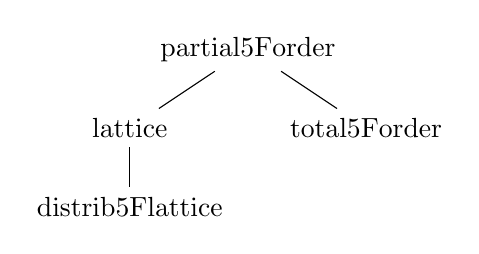
\begin{tikzpicture}
  \node (po) at (0,0) {\isa{partial{\isaliteral{5F}{\isacharunderscore}}order}};
  \node (lat) at (-1.5,-1) {\isa{lattice}};
  \node (dlat) at (-1.5,-2) {\isa{distrib{\isaliteral{5F}{\isacharunderscore}}lattice}};
  \node (to) at (1.5,-1) {\isa{total{\isaliteral{5F}{\isacharunderscore}}order}};
  \draw (po) -- (lat);
  \draw (lat) -- (dlat);
  \draw (po) -- (to);
%  \draw[->, dashed] (lat) -- (to);
\end{tikzpicture}
} \\
\subfigure[Total orders are lattices]{
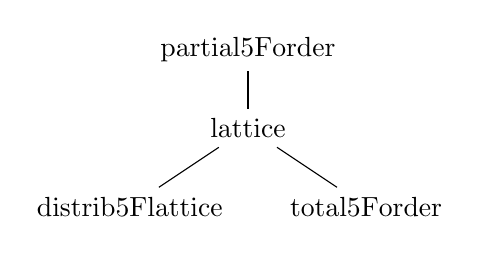
\begin{tikzpicture}
  \node (po) at (0,0) {\isa{partial{\isaliteral{5F}{\isacharunderscore}}order}};
  \node (lat) at (0,-1) {\isa{lattice}};
  \node (dlat) at (-1.5,-2) {\isa{distrib{\isaliteral{5F}{\isacharunderscore}}lattice}};
  \node (to) at (1.5,-2) {\isa{total{\isaliteral{5F}{\isacharunderscore}}order}};
  \draw (po) -- (lat);
  \draw (lat) -- (dlat);
  \draw (lat) -- (to);
%  \draw[->, dashed] (dlat) -- (to);
\end{tikzpicture}
} \quad
\subfigure[Total orders are distributive lattices]{
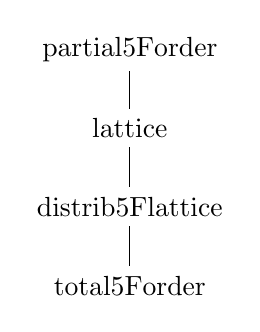
\begin{tikzpicture}
  \node (po) at (0,0) {\isa{partial{\isaliteral{5F}{\isacharunderscore}}order}};
  \node (lat) at (0,-1) {\isa{lattice}};
  \node (dlat) at (0,-2) {\isa{distrib{\isaliteral{5F}{\isacharunderscore}}lattice}};
  \node (to) at (0,-3) {\isa{total{\isaliteral{5F}{\isacharunderscore}}order}};
  \draw (po) -- (lat);
  \draw (lat) -- (dlat);
  \draw (dlat) -- (to);
\end{tikzpicture}
}
\end{center}
\hrule
\caption{Hierarchy of Lattice Locales.}
\label{fig:lattices}
\end{figure}%
\end{isamarkuptext}%
\isamarkuptrue%
%
\isamarkupsection{Changing the Locale Hierarchy
  \label{sec:changing-the-hierarchy}%
}
\isamarkuptrue%
%
\begin{isamarkuptext}%
Locales enable to prove theorems abstractly, relative to
  sets of assumptions.  These theorems can then be used in other
  contexts where the assumptions themselves, or
  instances of the assumptions, are theorems.  This form of theorem
  reuse is called \emph{interpretation}.  Locales generalise
  interpretation from theorems to conclusions, enabling the reuse of
  definitions and other constructs that are not part of the
  specifications of the locales.

  The first form of interpretation we will consider in this tutorial
  is provided by the \isakeyword{sublocale} command.  It enables to
  modify the import hierarchy to reflect the \emph{logical} relation
  between locales.

  Consider the locale hierarchy from Figure~\ref{fig:lattices}(a).
  Total orders are lattices, although this is not reflected here, and
  definitions, theorems and other conclusions
  from \isa{lattice} are not available in \isa{total{\isaliteral{5F}{\isacharunderscore}}order}.  To
  obtain the situation in Figure~\ref{fig:lattices}(b), it is
  sufficient to add the conclusions of the latter locale to the former.
  The \isakeyword{sublocale} command does exactly this.
  The declaration \isakeyword{sublocale} $l_1
  \subseteq l_2$ causes locale $l_2$ to be \emph{interpreted} in the
  context of $l_1$.  This means that all conclusions of $l_2$ are made
  available in $l_1$.

  Of course, the change of hierarchy must be supported by a theorem
  that reflects, in our example, that total orders are indeed
  lattices.  Therefore the \isakeyword{sublocale} command generates a
  goal, which must be discharged by the user.  This is illustrated in
  the following paragraphs.  First the sublocale relation is stated.%
\end{isamarkuptext}%
\isamarkuptrue%
%
\isadelimvisible
\ \ %
\endisadelimvisible
%
\isatagvisible
\isacommand{sublocale}\isamarkupfalse%
\ total{\isaliteral{5F}{\isacharunderscore}}order\ {\isaliteral{5C3C73756273657465713E}{\isasymsubseteq}}\ lattice%
\begin{isamarkuptxt}%
\normalsize
  This enters the context of locale \isa{total{\isaliteral{5F}{\isacharunderscore}}order}, in
  which the goal \begin{isabelle}%
\ {\isadigit{1}}{\isaliteral{2E}{\isachardot}}\ lattice\ op\ {\isaliteral{5C3C737173756273657465713E}{\isasymsqsubseteq}}%
\end{isabelle} must be shown.
  Now the
  locale predicate needs to be unfolded --- for example, using its
  definition or by introduction rules
  provided by the locale package.  For automation, the locale package
  provides the methods \isa{intro{\isaliteral{5F}{\isacharunderscore}}locales} and \isa{unfold{\isaliteral{5F}{\isacharunderscore}}locales}.  They are aware of the
  current context and dependencies between locales and automatically
  discharge goals implied by these.  While \isa{unfold{\isaliteral{5F}{\isacharunderscore}}locales}
  always unfolds locale predicates to assumptions, \isa{intro{\isaliteral{5F}{\isacharunderscore}}locales} only unfolds definitions along the locale
  hierarchy, leaving a goal consisting of predicates defined by the
  locale package.  Occasionally the latter is of advantage since the goal
  is smaller.

  For the current goal, we would like to get hold of
  the assumptions of \isa{lattice}, which need to be shown, hence
  \isa{unfold{\isaliteral{5F}{\isacharunderscore}}locales} is appropriate.%
\end{isamarkuptxt}%
\isamarkuptrue%
\ \ \isacommand{proof}\isamarkupfalse%
\ unfold{\isaliteral{5F}{\isacharunderscore}}locales%
\begin{isamarkuptxt}%
\normalsize
  Since the fact that both lattices and total orders are partial
  orders is already reflected in the locale hierarchy, the assumptions
  of \isa{partial{\isaliteral{5F}{\isacharunderscore}}order} are discharged automatically, and only the
  assumptions introduced in \isa{lattice} remain as subgoals
  \begin{isabelle}%
\ {\isadigit{1}}{\isaliteral{2E}{\isachardot}}\ {\isaliteral{5C3C416E643E}{\isasymAnd}}x\ y{\isaliteral{2E}{\isachardot}}\ {\isaliteral{5C3C6578697374733E}{\isasymexists}}inf{\isaliteral{2E}{\isachardot}}\ is{\isaliteral{5F}{\isacharunderscore}}inf\ x\ y\ inf\isanewline
\ {\isadigit{2}}{\isaliteral{2E}{\isachardot}}\ {\isaliteral{5C3C416E643E}{\isasymAnd}}x\ y{\isaliteral{2E}{\isachardot}}\ {\isaliteral{5C3C6578697374733E}{\isasymexists}}sup{\isaliteral{2E}{\isachardot}}\ is{\isaliteral{5F}{\isacharunderscore}}sup\ x\ y\ sup%
\end{isabelle}
  The proof for the first subgoal is obtained by constructing an
  infimum, whose existence is implied by totality.%
\end{isamarkuptxt}%
\isamarkuptrue%
\ \ \ \ \isacommand{fix}\isamarkupfalse%
\ x\ y\isanewline
\ \ \ \ \isacommand{from}\isamarkupfalse%
\ total\ \isacommand{have}\isamarkupfalse%
\ {\isaliteral{22}{\isachardoublequoteopen}}is{\isaliteral{5F}{\isacharunderscore}}inf\ x\ y\ {\isaliteral{28}{\isacharparenleft}}if\ x\ {\isaliteral{5C3C737173756273657465713E}{\isasymsqsubseteq}}\ y\ then\ x\ else\ y{\isaliteral{29}{\isacharparenright}}{\isaliteral{22}{\isachardoublequoteclose}}\isanewline
\ \ \ \ \ \ \isacommand{by}\isamarkupfalse%
\ {\isaliteral{28}{\isacharparenleft}}auto\ simp{\isaliteral{3A}{\isacharcolon}}\ is{\isaliteral{5F}{\isacharunderscore}}inf{\isaliteral{5F}{\isacharunderscore}}def{\isaliteral{29}{\isacharparenright}}\isanewline
\ \ \ \ \isacommand{then}\isamarkupfalse%
\ \isacommand{show}\isamarkupfalse%
\ {\isaliteral{22}{\isachardoublequoteopen}}{\isaliteral{5C3C6578697374733E}{\isasymexists}}inf{\isaliteral{2E}{\isachardot}}\ is{\isaliteral{5F}{\isacharunderscore}}inf\ x\ y\ inf{\isaliteral{22}{\isachardoublequoteclose}}\ \isacommand{{\isaliteral{2E}{\isachardot}}{\isaliteral{2E}{\isachardot}}}\isamarkupfalse%
%
\begin{isamarkuptxt}%
\normalsize
   The proof for the second subgoal is analogous and not
  reproduced here.%
\end{isamarkuptxt}%
\isamarkuptrue%
%
\endisatagvisible
{\isafoldvisible}%
%
\isadelimvisible
%
\endisadelimvisible
%
\isadeliminvisible
\ \ %
\endisadeliminvisible
%
\isataginvisible
\isacommand{next}\isamarkupfalse%
\isanewline
\ \ \ \ \isacommand{fix}\isamarkupfalse%
\ x\ y\isanewline
\ \ \ \ \isacommand{from}\isamarkupfalse%
\ total\ \isacommand{have}\isamarkupfalse%
\ {\isaliteral{22}{\isachardoublequoteopen}}is{\isaliteral{5F}{\isacharunderscore}}sup\ x\ y\ {\isaliteral{28}{\isacharparenleft}}if\ x\ {\isaliteral{5C3C737173756273657465713E}{\isasymsqsubseteq}}\ y\ then\ y\ else\ x{\isaliteral{29}{\isacharparenright}}{\isaliteral{22}{\isachardoublequoteclose}}\isanewline
\ \ \ \ \ \ \isacommand{by}\isamarkupfalse%
\ {\isaliteral{28}{\isacharparenleft}}auto\ simp{\isaliteral{3A}{\isacharcolon}}\ is{\isaliteral{5F}{\isacharunderscore}}sup{\isaliteral{5F}{\isacharunderscore}}def{\isaliteral{29}{\isacharparenright}}\isanewline
\ \ \ \ \isacommand{then}\isamarkupfalse%
\ \isacommand{show}\isamarkupfalse%
\ {\isaliteral{22}{\isachardoublequoteopen}}{\isaliteral{5C3C6578697374733E}{\isasymexists}}sup{\isaliteral{2E}{\isachardot}}\ is{\isaliteral{5F}{\isacharunderscore}}sup\ x\ y\ sup{\isaliteral{22}{\isachardoublequoteclose}}\ \isacommand{{\isaliteral{2E}{\isachardot}}{\isaliteral{2E}{\isachardot}}}\isamarkupfalse%
%
\endisataginvisible
{\isafoldinvisible}%
%
\isadeliminvisible
%
\endisadeliminvisible
%
\isadelimvisible
\ %
\endisadelimvisible
%
\isatagvisible
\isacommand{qed}\isamarkupfalse%
%
\endisatagvisible
{\isafoldvisible}%
%
\isadelimvisible
%
\endisadelimvisible
%
\begin{isamarkuptext}%
Similarly, we may establish that total orders are distributive
  lattices with a second \isakeyword{sublocale} statement.%
\end{isamarkuptext}%
\isamarkuptrue%
\ \ \isacommand{sublocale}\isamarkupfalse%
\ total{\isaliteral{5F}{\isacharunderscore}}order\ {\isaliteral{5C3C73756273657465713E}{\isasymsubseteq}}\ distrib{\isaliteral{5F}{\isacharunderscore}}lattice\isanewline
%
\isadelimproof
\ \ \ \ %
\endisadelimproof
%
\isatagproof
\isacommand{proof}\isamarkupfalse%
\ unfold{\isaliteral{5F}{\isacharunderscore}}locales\isanewline
\ \ \ \ \isacommand{fix}\isamarkupfalse%
\ x\ y\ z\isanewline
\ \ \ \ \isacommand{show}\isamarkupfalse%
\ {\isaliteral{22}{\isachardoublequoteopen}}x\ {\isaliteral{5C3C7371696E7465723E}{\isasymsqinter}}\ {\isaliteral{28}{\isacharparenleft}}y\ {\isaliteral{5C3C7371756E696F6E3E}{\isasymsqunion}}\ z{\isaliteral{29}{\isacharparenright}}\ {\isaliteral{3D}{\isacharequal}}\ x\ {\isaliteral{5C3C7371696E7465723E}{\isasymsqinter}}\ y\ {\isaliteral{5C3C7371756E696F6E3E}{\isasymsqunion}}\ x\ {\isaliteral{5C3C7371696E7465723E}{\isasymsqinter}}\ z{\isaliteral{22}{\isachardoublequoteclose}}\ {\isaliteral{28}{\isacharparenleft}}\isakeyword{is}\ {\isaliteral{22}{\isachardoublequoteopen}}{\isaliteral{3F}{\isacharquery}}l\ {\isaliteral{3D}{\isacharequal}}\ {\isaliteral{3F}{\isacharquery}}r{\isaliteral{22}{\isachardoublequoteclose}}{\isaliteral{29}{\isacharparenright}}%
\begin{isamarkuptxt}%
Jacobson I, p.\ 462%
\end{isamarkuptxt}%
\isamarkuptrue%
\ \ \ \ \isacommand{proof}\isamarkupfalse%
\ {\isaliteral{2D}{\isacharminus}}\isanewline
\ \ \ \ \ \ \isacommand{{\isaliteral{7B}{\isacharbraceleft}}}\isamarkupfalse%
\ \isacommand{assume}\isamarkupfalse%
\ c{\isaliteral{3A}{\isacharcolon}}\ {\isaliteral{22}{\isachardoublequoteopen}}y\ {\isaliteral{5C3C737173756273657465713E}{\isasymsqsubseteq}}\ x{\isaliteral{22}{\isachardoublequoteclose}}\ {\isaliteral{22}{\isachardoublequoteopen}}z\ {\isaliteral{5C3C737173756273657465713E}{\isasymsqsubseteq}}\ x{\isaliteral{22}{\isachardoublequoteclose}}\isanewline
\ \ \ \ \ \ \ \ \isacommand{from}\isamarkupfalse%
\ c\ \isacommand{have}\isamarkupfalse%
\ {\isaliteral{22}{\isachardoublequoteopen}}{\isaliteral{3F}{\isacharquery}}l\ {\isaliteral{3D}{\isacharequal}}\ y\ {\isaliteral{5C3C7371756E696F6E3E}{\isasymsqunion}}\ z{\isaliteral{22}{\isachardoublequoteclose}}\isanewline
\ \ \ \ \ \ \ \ \ \ \isacommand{by}\isamarkupfalse%
\ {\isaliteral{28}{\isacharparenleft}}metis\ c\ join{\isaliteral{5F}{\isacharunderscore}}connection{\isadigit{2}}\ join{\isaliteral{5F}{\isacharunderscore}}related{\isadigit{2}}\ meet{\isaliteral{5F}{\isacharunderscore}}related{\isadigit{2}}\ total{\isaliteral{29}{\isacharparenright}}\isanewline
\ \ \ \ \ \ \ \ \isacommand{also}\isamarkupfalse%
\ \isacommand{from}\isamarkupfalse%
\ c\ \isacommand{have}\isamarkupfalse%
\ {\isaliteral{22}{\isachardoublequoteopen}}{\isaliteral{2E}{\isachardot}}{\isaliteral{2E}{\isachardot}}{\isaliteral{2E}{\isachardot}}\ {\isaliteral{3D}{\isacharequal}}\ {\isaliteral{3F}{\isacharquery}}r{\isaliteral{22}{\isachardoublequoteclose}}\ \isacommand{by}\isamarkupfalse%
\ {\isaliteral{28}{\isacharparenleft}}metis\ meet{\isaliteral{5F}{\isacharunderscore}}related{\isadigit{2}}{\isaliteral{29}{\isacharparenright}}\isanewline
\ \ \ \ \ \ \ \ \isacommand{finally}\isamarkupfalse%
\ \isacommand{have}\isamarkupfalse%
\ {\isaliteral{22}{\isachardoublequoteopen}}{\isaliteral{3F}{\isacharquery}}l\ {\isaliteral{3D}{\isacharequal}}\ {\isaliteral{3F}{\isacharquery}}r{\isaliteral{22}{\isachardoublequoteclose}}\ \isacommand{{\isaliteral{2E}{\isachardot}}}\isamarkupfalse%
\ \isacommand{{\isaliteral{7D}{\isacharbraceright}}}\isamarkupfalse%
\isanewline
\ \ \ \ \ \ \isacommand{moreover}\isamarkupfalse%
\isanewline
\ \ \ \ \ \ \isacommand{{\isaliteral{7B}{\isacharbraceleft}}}\isamarkupfalse%
\ \isacommand{assume}\isamarkupfalse%
\ c{\isaliteral{3A}{\isacharcolon}}\ {\isaliteral{22}{\isachardoublequoteopen}}x\ {\isaliteral{5C3C737173756273657465713E}{\isasymsqsubseteq}}\ y\ {\isaliteral{5C3C6F723E}{\isasymor}}\ x\ {\isaliteral{5C3C737173756273657465713E}{\isasymsqsubseteq}}\ z{\isaliteral{22}{\isachardoublequoteclose}}\isanewline
\ \ \ \ \ \ \ \ \isacommand{from}\isamarkupfalse%
\ c\ \isacommand{have}\isamarkupfalse%
\ {\isaliteral{22}{\isachardoublequoteopen}}{\isaliteral{3F}{\isacharquery}}l\ {\isaliteral{3D}{\isacharequal}}\ x{\isaliteral{22}{\isachardoublequoteclose}}\isanewline
\ \ \ \ \ \ \ \ \ \ \isacommand{by}\isamarkupfalse%
\ {\isaliteral{28}{\isacharparenleft}}metis\ join{\isaliteral{5F}{\isacharunderscore}}connection{\isadigit{2}}\ join{\isaliteral{5F}{\isacharunderscore}}related{\isadigit{2}}\ meet{\isaliteral{5F}{\isacharunderscore}}connection\ total\ trans{\isaliteral{29}{\isacharparenright}}\isanewline
\ \ \ \ \ \ \ \ \isacommand{also}\isamarkupfalse%
\ \isacommand{from}\isamarkupfalse%
\ c\ \isacommand{have}\isamarkupfalse%
\ {\isaliteral{22}{\isachardoublequoteopen}}{\isaliteral{2E}{\isachardot}}{\isaliteral{2E}{\isachardot}}{\isaliteral{2E}{\isachardot}}\ {\isaliteral{3D}{\isacharequal}}\ {\isaliteral{3F}{\isacharquery}}r{\isaliteral{22}{\isachardoublequoteclose}}\isanewline
\ \ \ \ \ \ \ \ \ \ \isacommand{by}\isamarkupfalse%
\ {\isaliteral{28}{\isacharparenleft}}metis\ join{\isaliteral{5F}{\isacharunderscore}}commute\ join{\isaliteral{5F}{\isacharunderscore}}related{\isadigit{2}}\ meet{\isaliteral{5F}{\isacharunderscore}}connection\ meet{\isaliteral{5F}{\isacharunderscore}}related{\isadigit{2}}\ total{\isaliteral{29}{\isacharparenright}}\isanewline
\ \ \ \ \ \ \ \ \isacommand{finally}\isamarkupfalse%
\ \isacommand{have}\isamarkupfalse%
\ {\isaliteral{22}{\isachardoublequoteopen}}{\isaliteral{3F}{\isacharquery}}l\ {\isaliteral{3D}{\isacharequal}}\ {\isaliteral{3F}{\isacharquery}}r{\isaliteral{22}{\isachardoublequoteclose}}\ \isacommand{{\isaliteral{2E}{\isachardot}}}\isamarkupfalse%
\ \isacommand{{\isaliteral{7D}{\isacharbraceright}}}\isamarkupfalse%
\isanewline
\ \ \ \ \ \ \isacommand{moreover}\isamarkupfalse%
\ \isacommand{note}\isamarkupfalse%
\ total\isanewline
\ \ \ \ \ \ \isacommand{ultimately}\isamarkupfalse%
\ \isacommand{show}\isamarkupfalse%
\ {\isaliteral{3F}{\isacharquery}}thesis\ \isacommand{by}\isamarkupfalse%
\ blast\isanewline
\ \ \ \ \isacommand{qed}\isamarkupfalse%
\isanewline
\ \ \isacommand{qed}\isamarkupfalse%
%
\endisatagproof
{\isafoldproof}%
%
\isadelimproof
%
\endisadelimproof
%
\begin{isamarkuptext}%
The locale hierarchy is now as shown in
  Figure~\ref{fig:lattices}(c).%
\end{isamarkuptext}%
\isamarkuptrue%
%
\begin{isamarkuptext}%
Locale interpretation is \emph{dynamic}.  The statement
  \isakeyword{sublocale} $l_1 \subseteq l_2$ will not just add the
  current conclusions of $l_2$ to $l_1$.  Rather the dependency is
  stored, and conclusions that will be
  added to $l_2$ in future are automatically propagated to $l_1$.
  The sublocale relation is transitive --- that is, propagation takes
  effect along chains of sublocales.  Even cycles in the sublocale relation are
  supported, as long as these cycles do not lead to infinite chains.
  Details are discussed in the technical report \cite{Ballarin2006a}.
  See also Section~\ref{sec:infinite-chains} of this tutorial.%
\end{isamarkuptext}%
\isamarkuptrue%
%
\isadelimtheory
%
\endisadelimtheory
%
\isatagtheory
\isacommand{end}\isamarkupfalse%
%
\endisatagtheory
{\isafoldtheory}%
%
\isadelimtheory
%
\endisadelimtheory
\isanewline
\end{isabellebody}%
%%% Local Variables:
%%% mode: latex
%%% TeX-master: "root"
%%% End:
